\chapter{User Interfaces and Implementing Multiple Game Modes}

So far we have made a lot of progress on the core mechanic of our game. Another
important aspect are the screens and components that wrap this mechanic. In this chapter
you will learn how to implement menus, popups and other user interface elements
in \cocos{}. 

Throughout this chapter you will not only learn how to build user interfaces
with \cocos{} and \SB{}, you will also learn how to structure this game to
support two different gameplay modes. We will implement and \textit{endless} and
a \textit{timed} gameplay mode, each with a different set of rules and
behaviors. We will choose an architecture that will make it easy to add more
game modes in future.

By the end of this chapter we will have a fully functional game!
Here's the basic screen flow our game will have:

\begin{figure}[H]
		\centering
		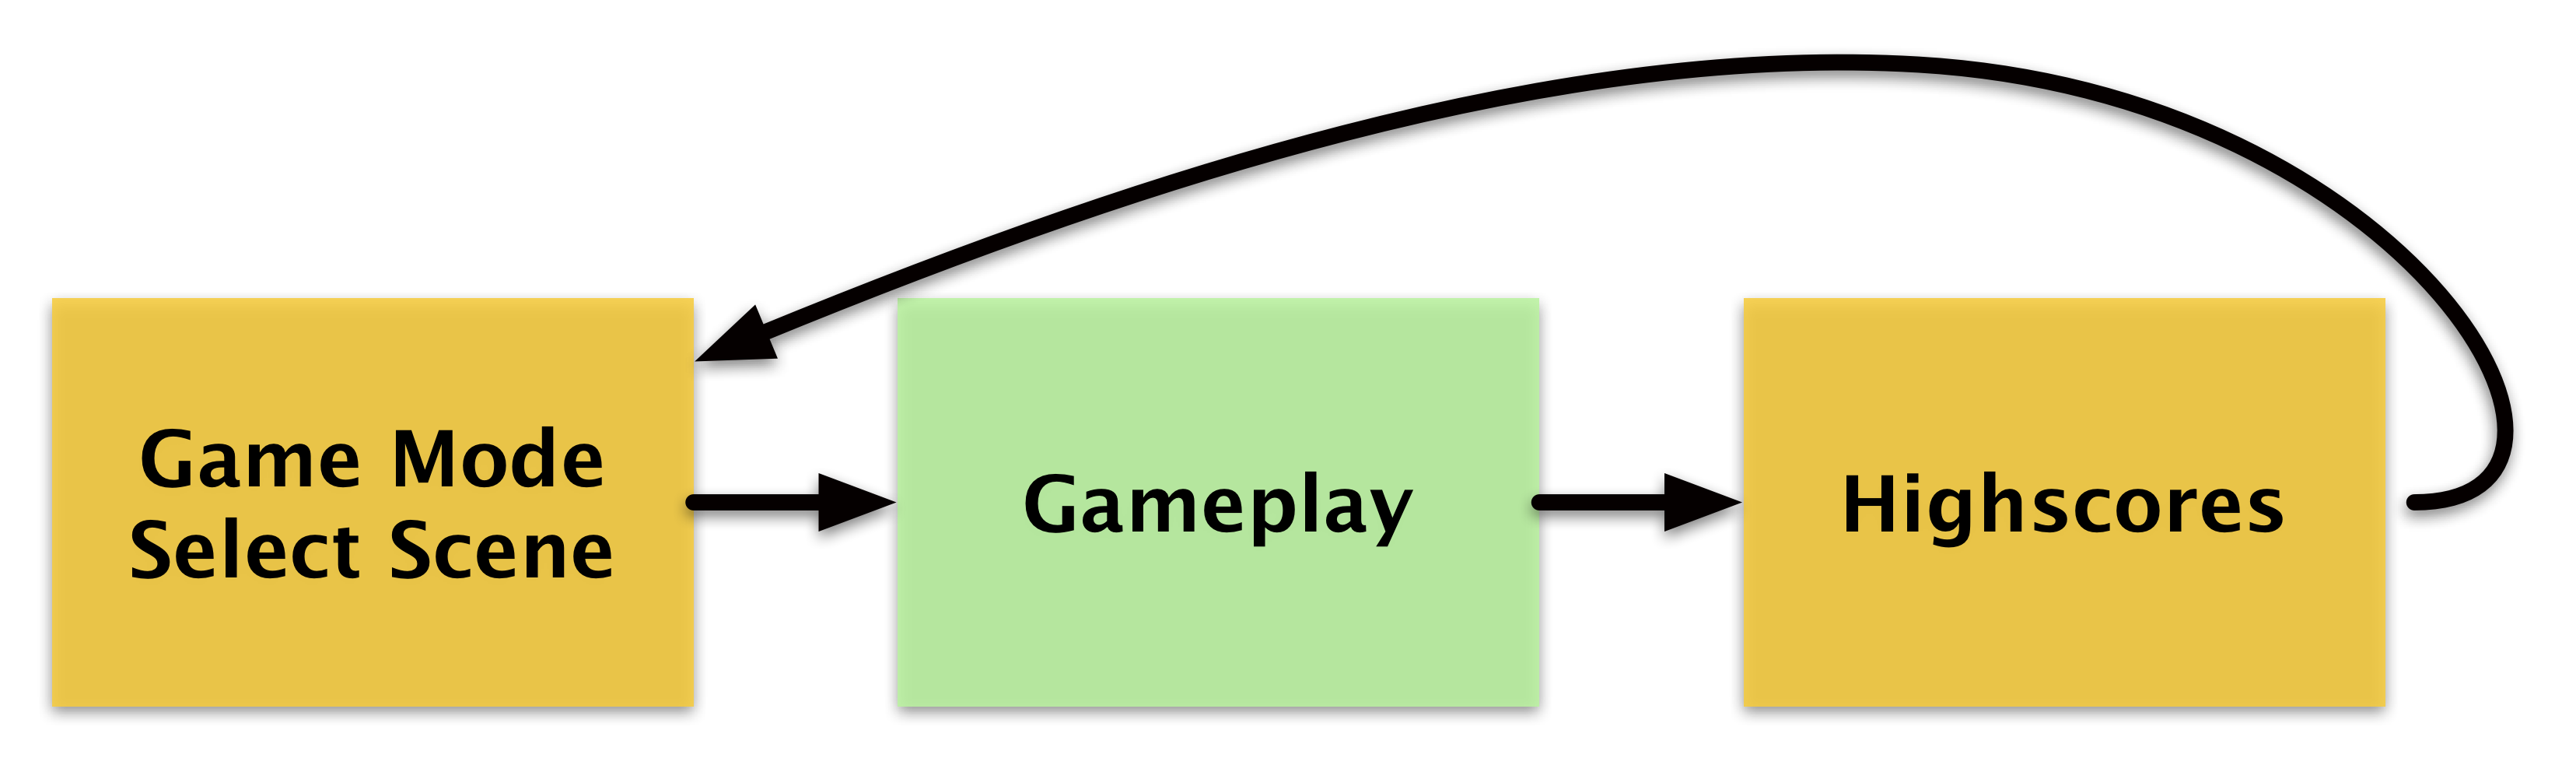
\includegraphics[width=0.7\linewidth]{images/Chapter6/screen_flow.png}
\end{figure}

Let's start out by adding the game mode selection scene!

\section{Adding a Game Mode Selection Scene}
We will now change the screen flow of our existing game. Instead of diving into
the gameplay directly the user will see a game mode selection scene when
starting the game. 

The game mode selection scene will allow the user to swipe to switch between the
endless and timed game mode. Luckily \cocos{} provides a component called
\inlinecode{CCScrollView}\index{User Interface!CCScrollView} that implements
most of the functionality that we need for that scene.

\subsection{Setting the Start Scene Up}

\begin{leftbar}
Open the \SB{} project and create a new File (File -> New -> File\ldots). Name
the new file \textit{StartScene} and select \textit{Scene} as the type.
\end{leftbar}

We will create a game mode select scene that smoothly transitions into the
gameplay. To accomplish that we'll use the same background image for this scene
as for the actual gameplay. 

\begin{leftbar}
Drag the image \textit{backround.png} image onto the stage; it becomes the first
child of the root node of our new \textit{StartScene}.
\end{leftbar}

The background image should have exactly the same settings as in
\textit{MainScene} so that it fills the entire scene.

\begin{leftbar}
Select the background sprite in the timeline and apply the following steps:
\begin{enumerate}
  \item Set the \textit{Position type} for X and Y to \textit{percent of parent
  container}
  \item Set the \textit{Position} to \textit{(50, 50)}
\end{enumerate}
\end{leftbar}

Now the background image should fill the entire background. We will be
presenting some information in front of that background. To make that
information stand out more we will dim the background a little bit by turning
down its opacity. Since the default fill color behind the background image is
black, a lower opacity will result in a darker image.

\begin{leftbar}
Select the background sprite in the timeline. Set the opacity in the property
inspector to \textit{0.7}:
\begin{figure}[H]
		\centering
		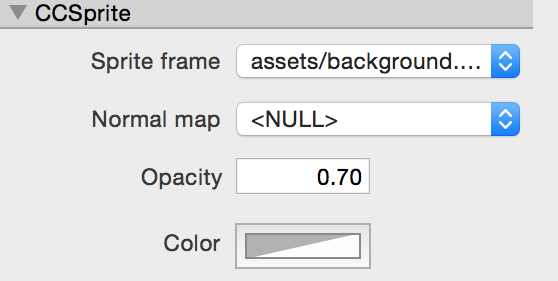
\includegraphics[width=200pt]{images/Chapter6/opacity_lower.png}
\end{figure}
\end{leftbar}

Next, we are going to add a label with an instruction for the player. A label is
a simple UI component that can display text. When building games with \cocos{}
we want to place the most UI components relative to screen edges. Using this
approach the UI will still look good when the game runs on a device with a
different screen size. Here's a little illustration:

\begin{figure}[H]
		\centering
		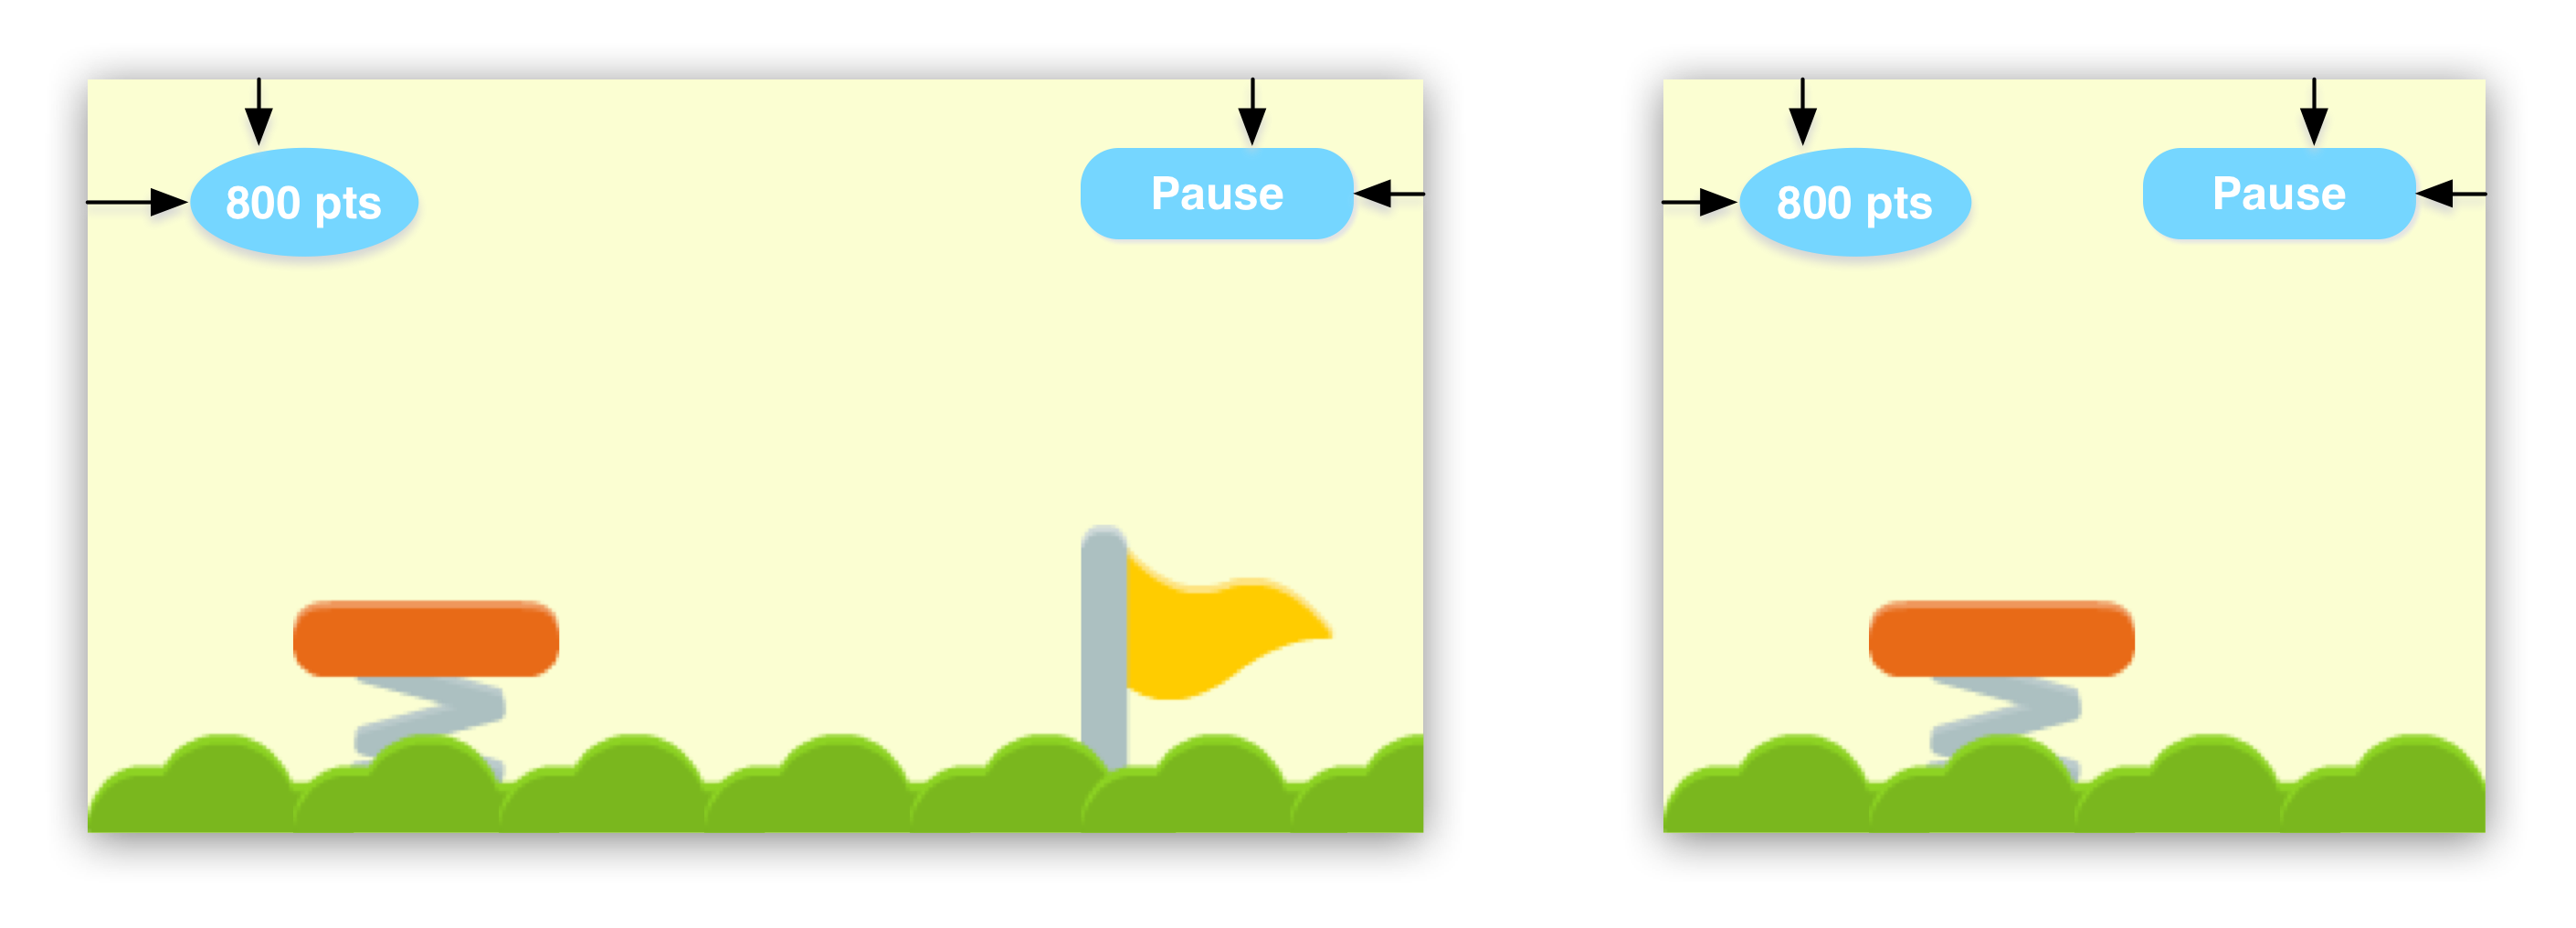
\includegraphics[width=0.7\linewidth]{images/Chapter6/multiple_screen_sizes.png}
		\caption{UI elements should be placed relative to screen edges to preserve
		their position on different screen sizes}
\end{figure}

As the screen resizes, the visible portion of the gameplay changes while the
button positions remain similar.

Throughout this chapter we will use \cocos{}'s reference
corner feature to accomplish resizable user interfaces. 

\begin{leftbar}
Drag a \textit{CCLabelTTF} from the node library \textit{below} the background
sprite, so that is rendered on top of the background image:
\begin{figure}[H]
    \centering
    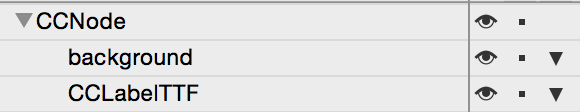
\includegraphics[width=200pt]{images/Chapter7/label_ontop_background.png}
\end{figure}
 
Set the position up as following:
\begin{enumerate}
  \item Set the \textit{Position Reference Corner} to \textit{Top-left}:
  \begin{figure}[H]
    \centering
    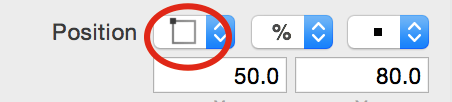
\includegraphics[width=130pt]{images/Chapter7/pos_ref_corner.png}
\end{figure}
  \item Set the position type for X to \textit{percent of parent container}
  \item Set the X position to \textit{50}
  \item Set the Y position to \textit{80}
\end{enumerate}

Set the label text to: \textit{Choose your game mode:}. We also want to change
the font and appearance of this label a little:
\begin{enumerate}
  \item As font name choose: \textit{Optima-Bold}
  \item As font size choose: \textit{40}
  \item Under \textit{Font Effects}, set the draw color to \textit{black}
  \item Set the outline color to \textit{white}
  \item Set the outline width to \textit{6}
\end{enumerate}
\end{leftbar}

After setting the label up your start scene should look as following:

\begin{figure}[H]
		\centering
		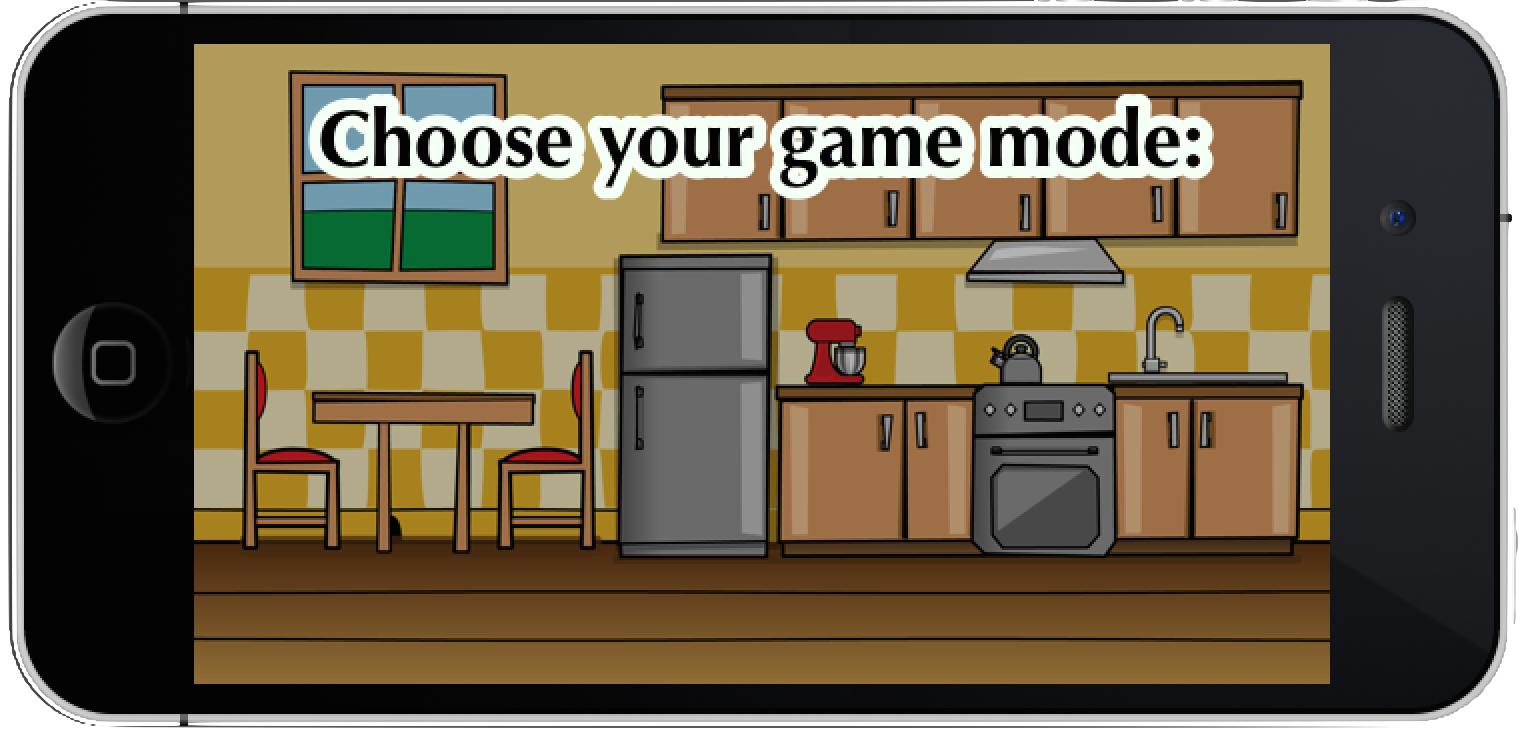
\includegraphics[width=0.7\linewidth]{images/Chapter7/start_scene.png}
\end{figure}

There's a lot more work left to do! As mentioned earlier we will create a scroll
view that let's the user swipe between two different game modes. Every scroll
view has a content node. That content node is larger than the size of the scroll
view and the scroll view can be used to view different parts of this content
node. Here's an illustration:

\begin{figure}[H]
		\centering
		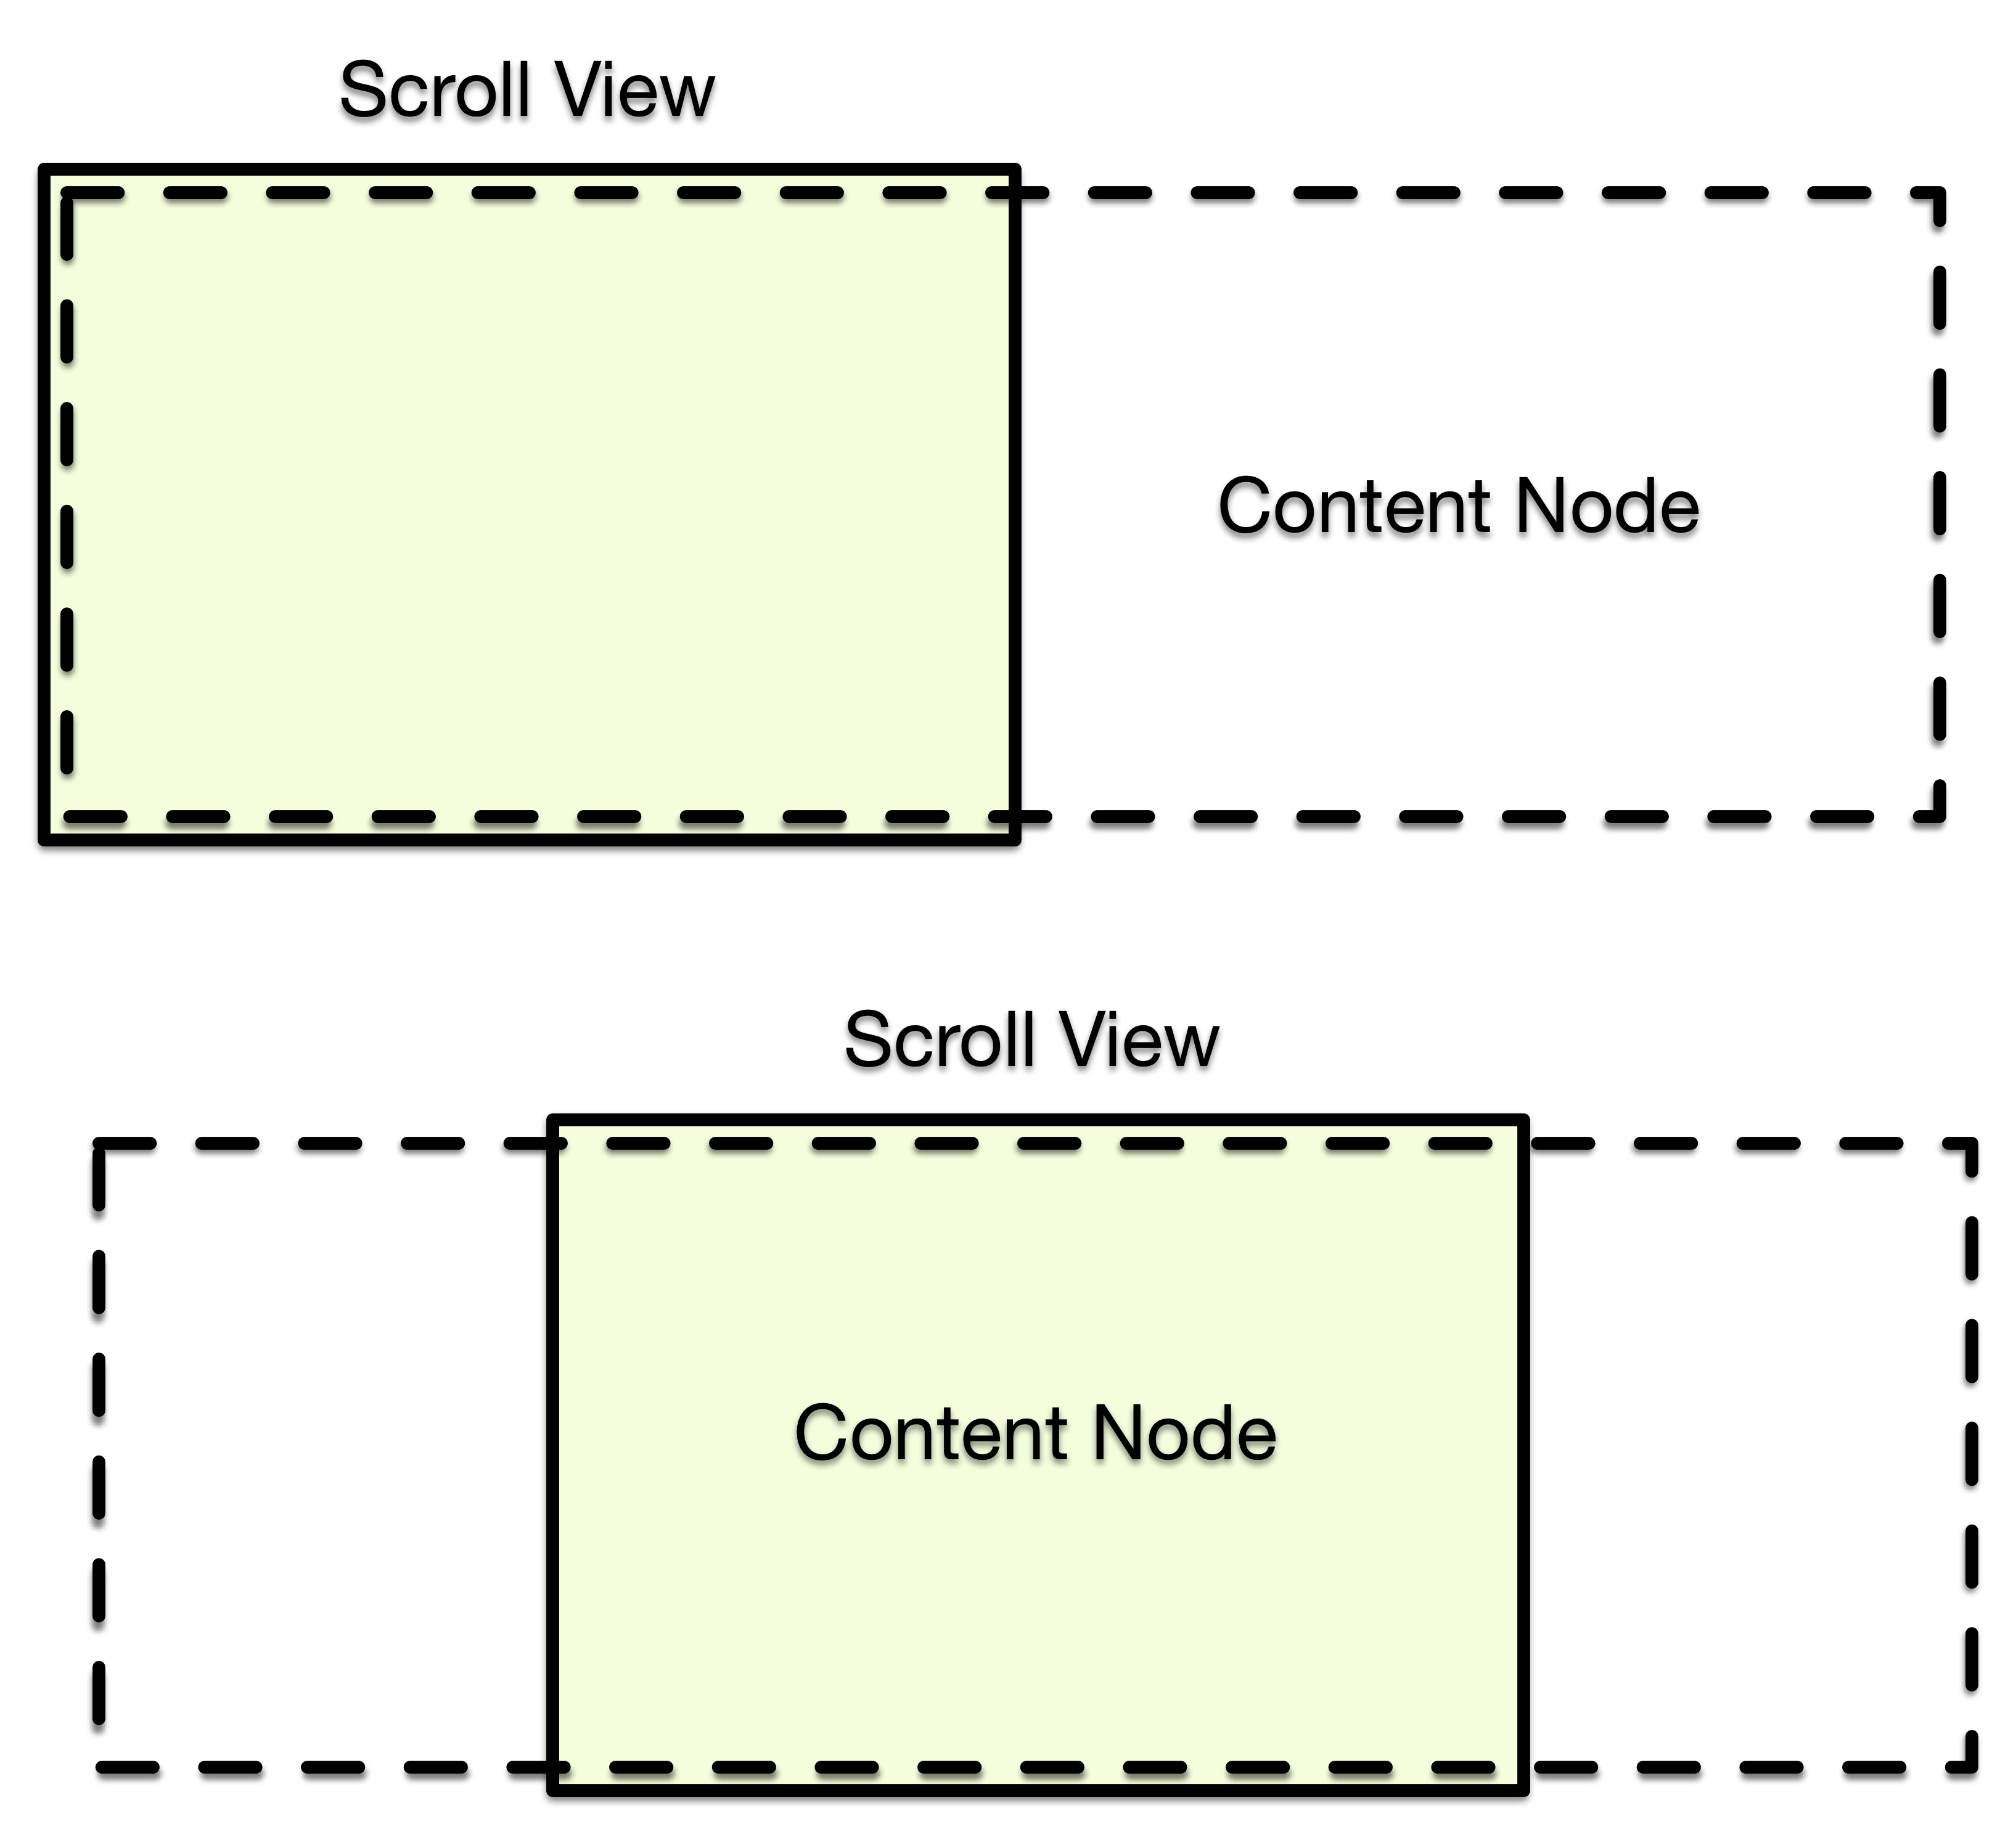
\includegraphics[width=0.5\linewidth]{images/Chapter7/scrollview_concept.png}
		\caption{The scroll view can present different portions of its larger content
		node. The user can change the displayed portion by swiping.}
\end{figure}

Our next step will be creating this content node. In general scroll views allow
users to scroll to any arbitrary position within the scroll view's content node.
In our specific example we would like to change this behavior. We only
want the user to select between two different game modes, each of these game modes will be
represented by a full screen node. It wouldn't make sense to allow the user to
scroll half way between the endless and timed game mode. For this specific case
the scroll view provides an option called \textit{Paging enabled}. If you want
to use a scroll view with paging, your content node needs to have a size that is
a multiple of the scroll view's size. In our particular example the content node
for our scroll view will be twice as wide as the scroll view itself, resulting
in a scroll view with two pages. When paging is enabled, the scroll view will
always snap to one of the two pages as soon as a user stops scrolling. If this
sounds a little bit too abstract for you, it should become clearer as we implement and use the scroll view.

\subsection{Creating the Content Node for the Scroll View}

First we need to create the content view. We will set it up in a separate
\ccbfile{} file. 
\begin{leftbar}
Create a new \ccbfile{} called \textit{GameModeSelectLayer} and choose its type
to be a \textit{Layer}.
\end{leftbar}

\begin{details}[Why are we using a Layer to create the scroll view
content?]\index{Document Types}
A short refresher on the different \ccbfile{} types: Scenes are used to
represent full screen content. Sprites are used for simple Sprite Images. Nodes
are used for node compositions that don't have a specific content size. Layers
are used to create content within a stage that has a fixed size.
Layers are typically used for popups or scroll view content nodes because we
want to layout the content based on a container size. We can still use
parent-relative sizing for layers. For our scroll view content layer we will set
a width that is \textit{2x} the width of the parent container. As soon as that
layer is added to another node, the final size of it will be determined based on
the size of that parent node.
\end{details}

\begin{leftbar}
Change the size of the root node:
\begin{enumerate}
  \item Select the root node of \textit{GameModeSelectLayer.ccb}
  \item Set the \textit{Content Size Type} of the width and height to  
  \textit{percent of the parent container}
  \item Set the content size to \textit{(200, 100)}
\end{enumerate}
\begin{figure}[H]
		\centering
		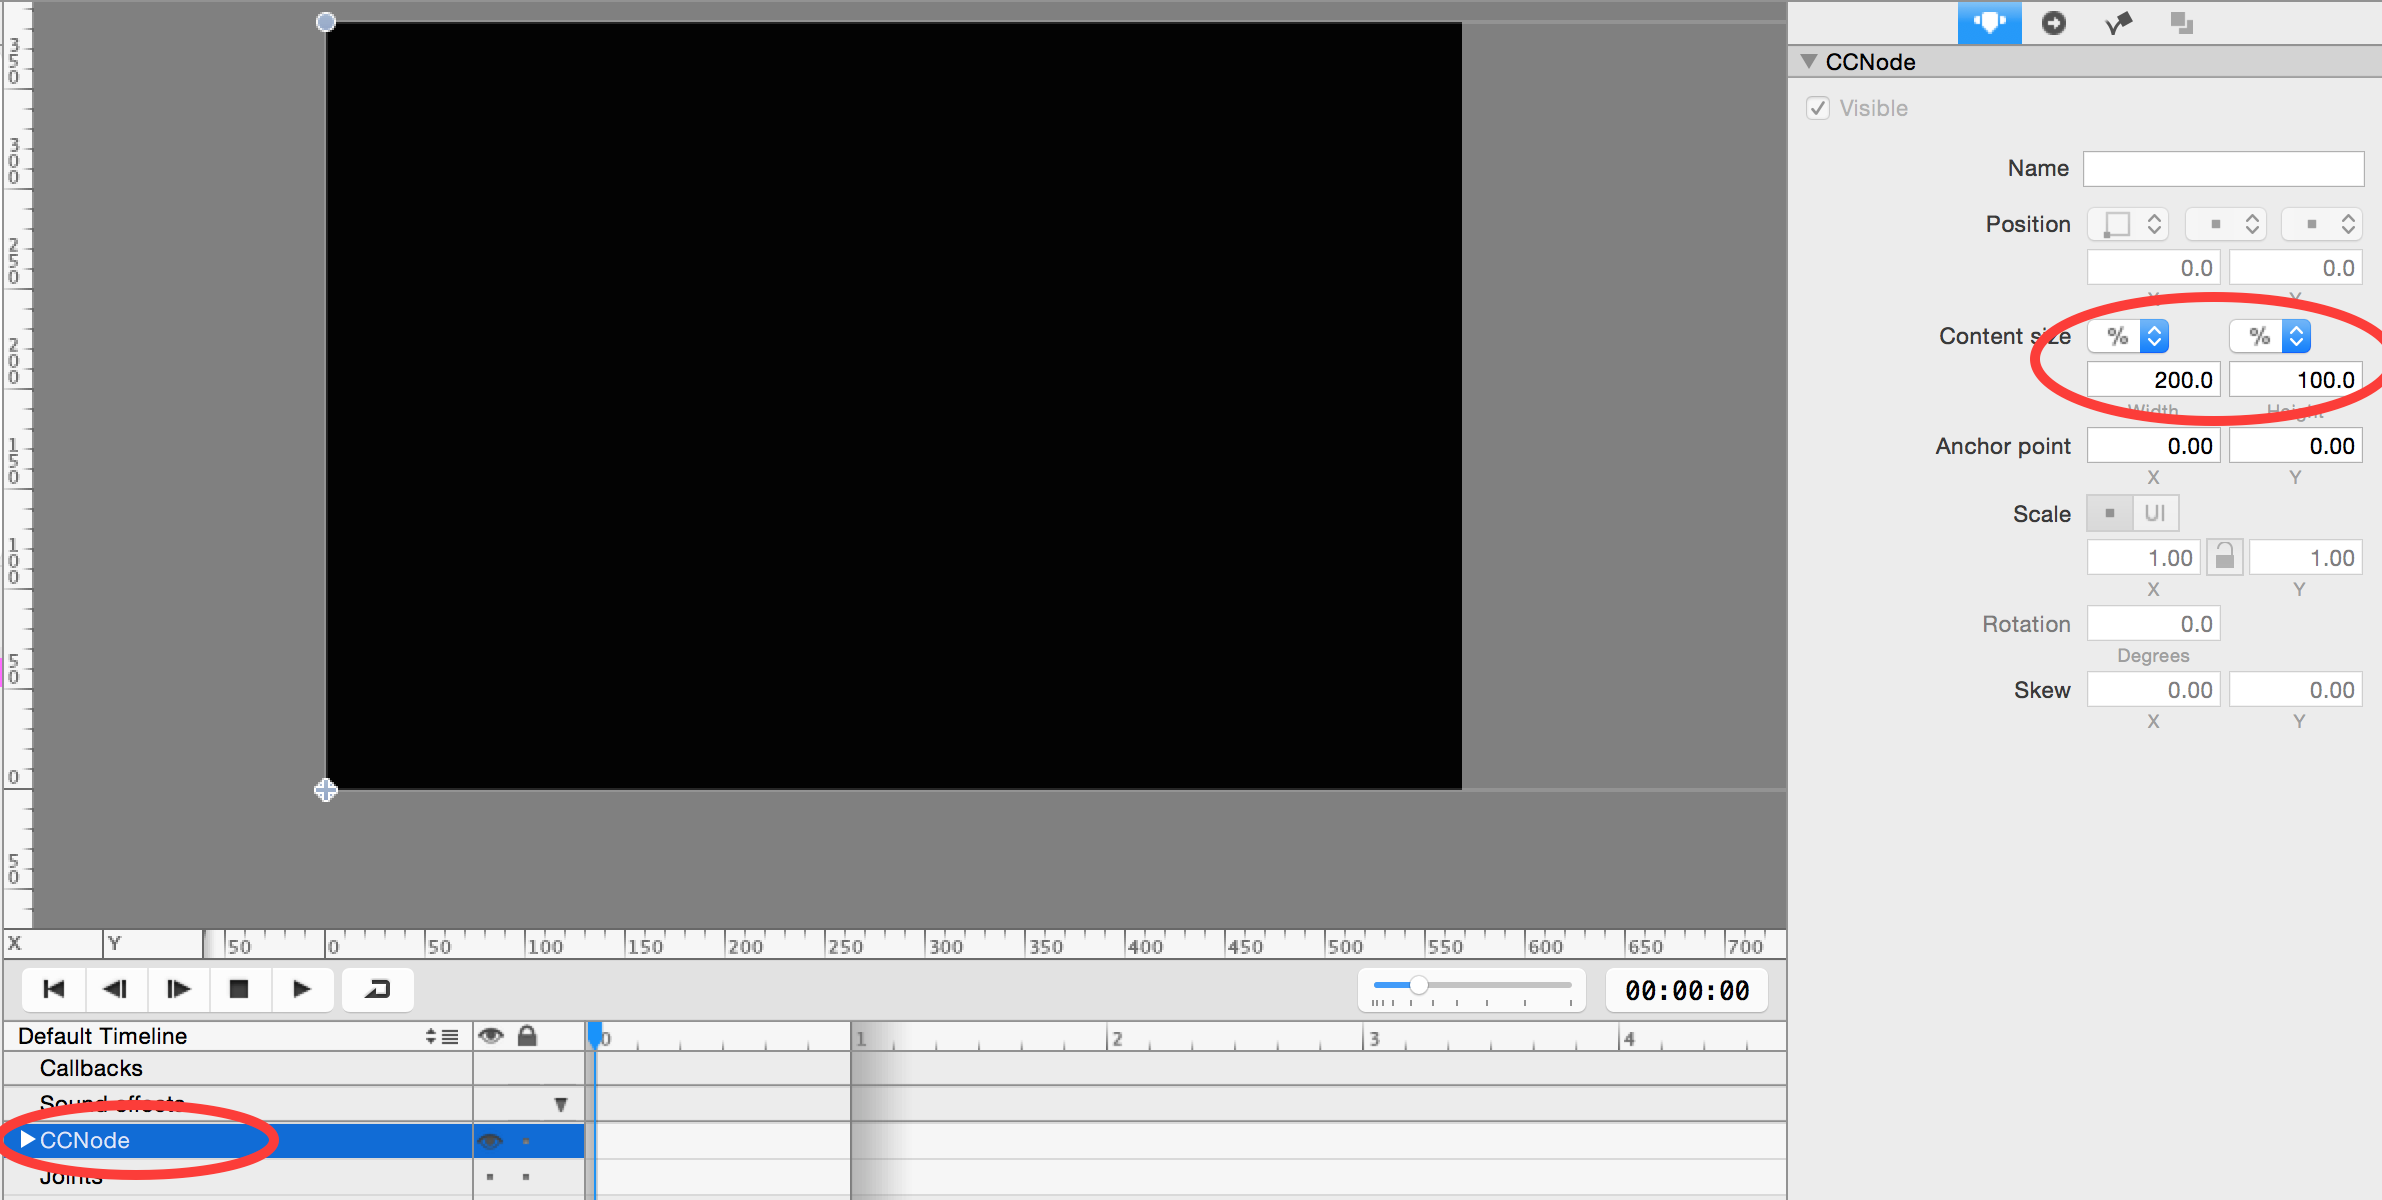
\includegraphics[width=0.85\linewidth]{images/Chapter7/content_node_width.png}
\end{figure}
\end{leftbar}

We want the scroll view to contain two pages, that means the content node needs
to be exactly double as wide as the scroll view. Because we are setting up the
size of the root node of this \ccbfile{} in percentage of the parent container,
its actual size will only be determined when it is added to a scroll view. This
is a great example of dynamic layouts; our scroll view could have any
arbitrary size and this content node would always be exactly twice as wide.

Inside of this root node we are going to place the content for our two different
pages. To provide a clean structure we will create one container node for each
page.

\begin{leftbar}
Add the container node for the left page:
\begin{enumerate}
  \item Add a plain \ccnode{} as a child to the root node of
  \filemention{GameModeSelectLayer.ccb}
  \item Name this child \textit{endless-mode} by selecting the node in the timeline and
 hitting the return key
  \item Set the \textit{Content Size Type} to \textit{Percent of parent
  container} for both \textit{Width} and \textit{Height}
  \item Set the \textit{Content Size} to \textit{(50, 100)}
\end{enumerate}
\end{leftbar}

The first page is set up; let's add the second one.

\begin{leftbar}
Add the container node for the right page:
\begin{enumerate}
  \item Add a plain \ccnode{} as a child to the root node of
  \filemention{GameModeSelectLayer.ccb}
  \item Name this child \textit{timed-mode} by selecting the node in the
  timeline and hitting the return key
  \item Set the \textit{Content Size Type} to \textit{Percent of parent
  container} for both \textit{Width} and \textit{Height}
  \item Set the \textit{Content Size} to \textit{(50, 100)}
  \item Additionally, set the \textit{Position Type} for \textit{X} to
  \textit{Percent of parent container}
  \item Set the \textit{Position} to \textit{(50, 0)}
\end{enumerate}
\end{leftbar}

Now we have containers for each page set up. We are going to fill them with
labels that describe the game mode represented on each page. We'll also add an
arrow indicating that there is another game mode available by swiping across the
screen. This is what the completed content node will look like:

\begin{figure}[H]
		\centering
		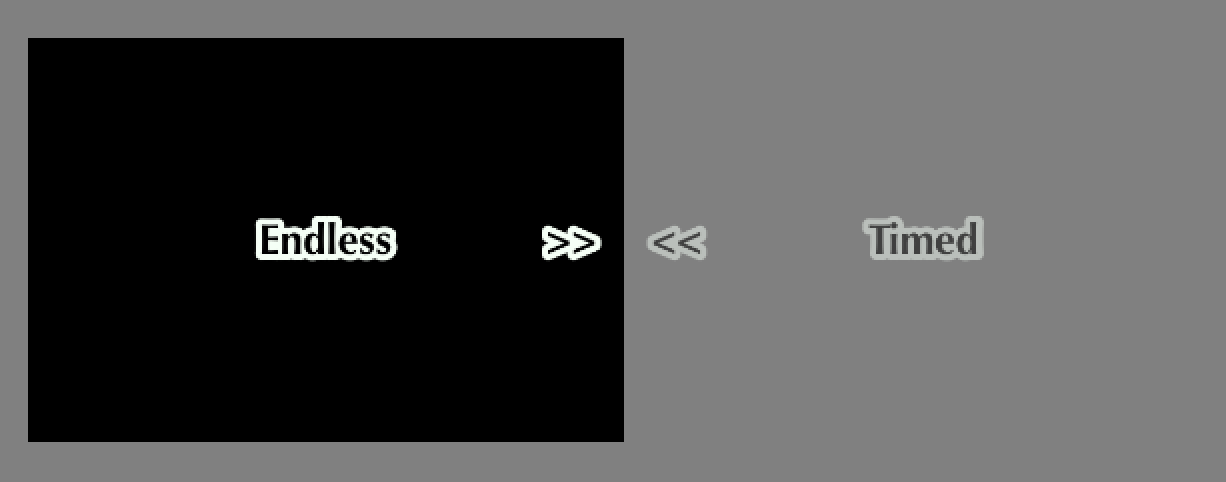
\includegraphics[width=0.6\linewidth]{images/Chapter7/content_node_completed.png}
		\caption{The completed content node by the end of this section.}
\end{figure}

First, let's add the labels for the endless mode.

\begin{leftbar}
Add the label for the endless mode, it should ook the same as the \textit{Choose your game mode} label on the start
scene:
\begin{enumerate}
  \item Drag a \cclabel{} from the node library onto the \textit{endless-mode}
  node
  \item Center the label within its parent node by choosing a \textit{Position type} of
\textit{percentage of parent container}
  \item Set the \textit{Position} to \textit{(50, 50)} 
  \item Set the label text to \textit{Endless}
  \item As font name choose: \textit{Optima-Bold}
  \item As font size choose: \textit{40}
  \item Set the draw color to \textit{black}
  \item Set the outline color to \textit{white}
  \item Set the outline width to \textit{6}
\end{enumerate}
\end{leftbar}

Next, let's add the arrow on the right side that will indicate that the player
can switch to the timed game mode.

\begin{leftbar}
Add an arrow to the \textit{endless-mode} node:
\begin{enumerate}
  \item Copy and Past the \textit{Endless} node
  \item Change the label text to \textit{>>}
  \item Set the position up as following: \begin{figure}[H]
										  \centering
										  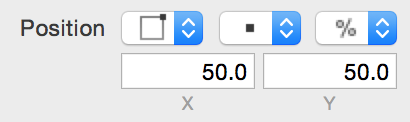
\includegraphics[width=150pt]{images/Chapter7/arrow_label_position.png}
										  \end{figure}
\end{enumerate}
\end{leftbar}

Now your stage should look like this:
\begin{figure}[H]
\centering
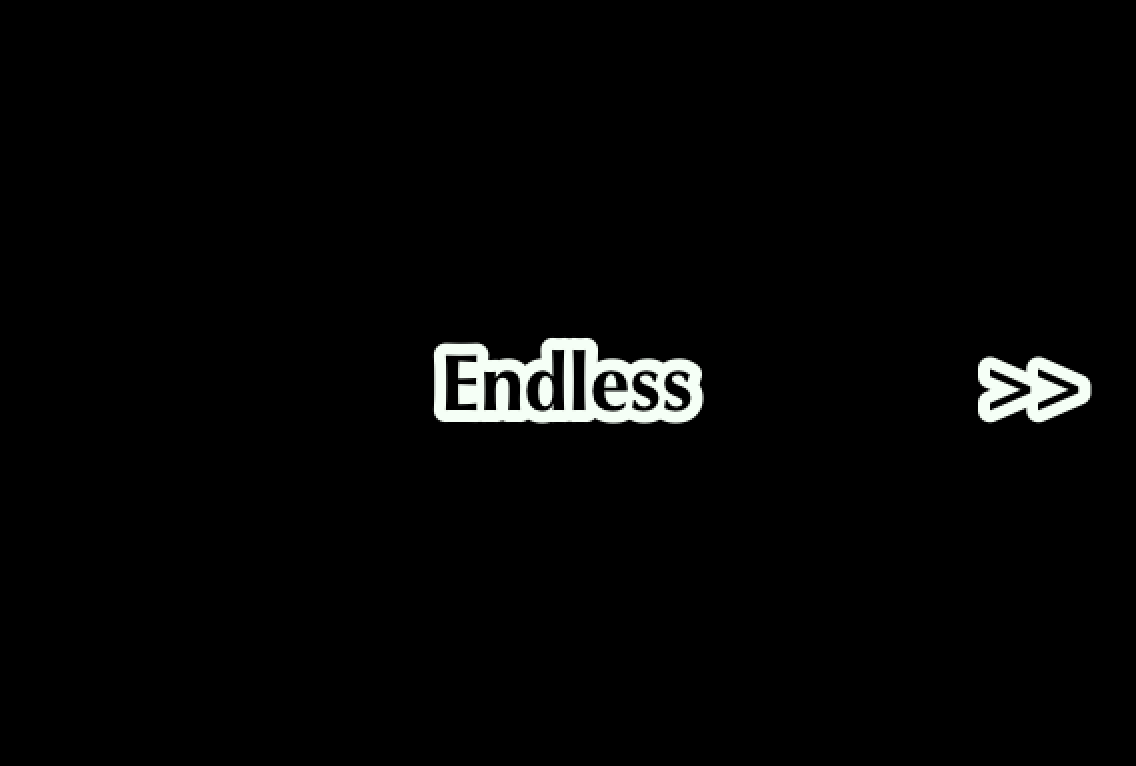
\includegraphics[width=150pt]{images/Chapter7/endless_mode.png}
\end{figure}
We're going to add a little visual detail to this game mode selection layer. The
arrows indicating the other available game mode shall blink. This can be easily
accomplished using \SB{}'s timeline feature. The animation shall last one
second, so start by changing the timeline duration.

\begin{leftbar}
Set the timeline duration to 1 second as illustrated in the image below: 
\begin{figure}[H]
\centering
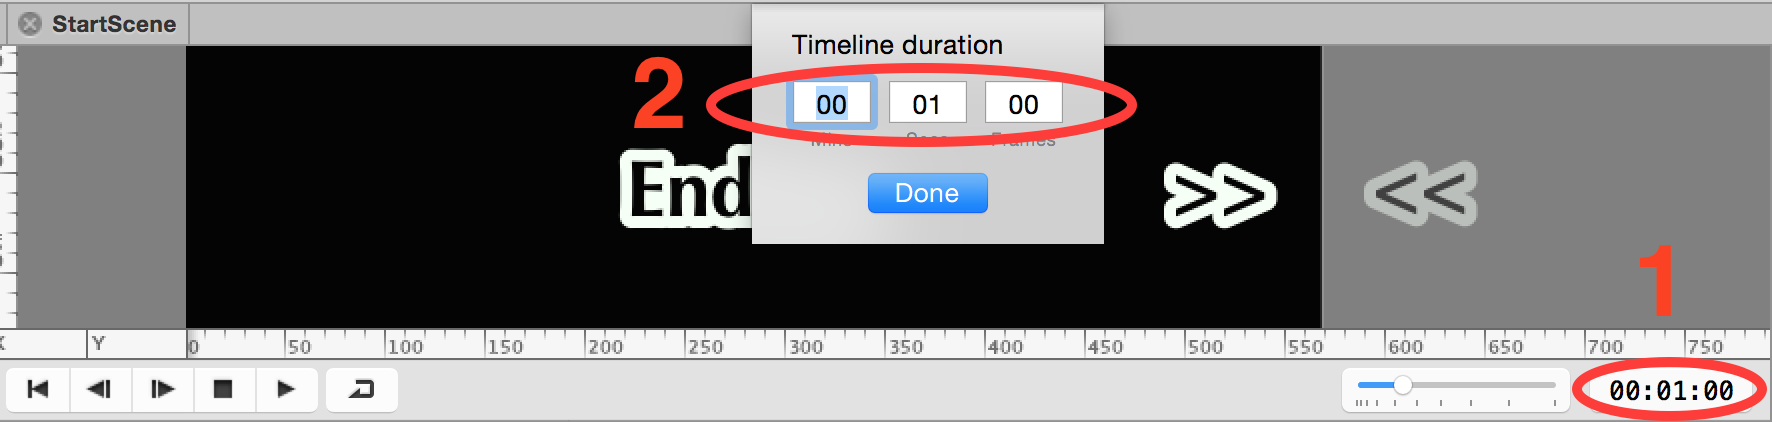
\includegraphics[width=300pt]{images/Chapter7/timeline_duration.png}
\caption{Changing the timeline duration}\label{fig:
timeline_duration}\index{SpriteBuilder Timeline!Change Duration}
\end{figure}
\end{leftbar}

Now we are going to use three \textit{opacity} keyframes to create the blinking
animation. 
\begin{leftbar}
Select the label with the arrows in the timeline. Then create three
keyframes. Place the first keyframe
at timestamp 00:00:00 the second one at timestamp 00:00:15 and the third
one at timestamp 00:01:00. You can choose the exact position of a
keyframe by dragging the timeline ruler to the according position. You can create keyframes by hitting the
\textit{O} (like in opacity) key on your keyboard. Alternatively you can create
keyframes through the top bar menu:
\textit{Animation -> Insert Keyframe\ldots -> Opacity}:
\begin{figure}[H]
\centering
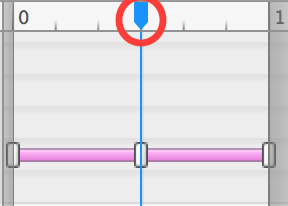
\includegraphics[width=70pt]{images/Chapter7/timeline_ruler.png}
\caption{Drag the timeline ruler to select a frame at which you want to create
the keyframe}
\end{figure}
\end{leftbar}

Now we can set different opacity values for each of these keyframes and \SB{}
will create smooth animations between them. There are two ways to set a
specific value for a keyframe. You can select the keyframe and change the
relevant property in the property inspector in the right panel of \SB{}. The
easier way however is to double-click onto a keyframe. That will bring up a
small popup in which you can modify the relevant values:
\begin{figure}[H]
\centering
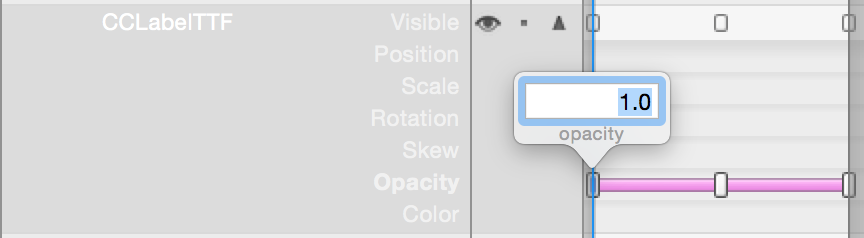
\includegraphics[width=250pt]{images/Chapter7/edit_keyframe.png}
\caption{Double-click onto keyframes to modify their values}
\end{figure}

\begin{leftbar}
Set the opacity in the first keyframe to 1.0. Set the opacity to 0.0 in the
second keyframe. For the third keyframe set the opacity to 1.0 again.
\end{leftbar}

Now the arrow will appear for half a second and then disappear for another half
a second. We don't want this animation to be over after 1 second. Instead we
want to loop it forever. We can do so by \textit{chaining}\index{\SB{}
Timeline!Chaining} the timeline to itself. In \SB{} timelines can be chained to
each other. That means that you can define that another timeline should run
after the current timeline is completed. If you use this feature to chain a
timeline to itself you have an endlessly running timeline animation!

\begin{leftbar}
Chain the default timeline to itself as shown below:
\begin{figure}[H]
\centering
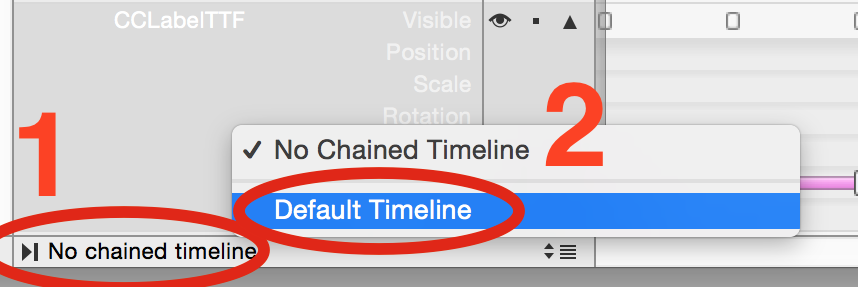
\includegraphics[width=200pt]{images/Chapter7/chain_timeline_2.png}
\caption{\SB{} allows you to connect different animations by chaining
timelines}
\end{figure}
\end{leftbar}

\begin{details}[Looping animations in \SB{}]
Animations that are set up with a chained timeline will loop endlessly when your
game is running on a simulator or phone. In \SB{} itself the animation will only
run once. If you want to preview what your animation will look like when it is
looped, you need to use the following control in the timeline playback panel:
\begin{figure}[H]
\centering

\includegraphics[width=100pt]{images/Chapter7/loop_timeline.png}
\end{figure}
Note that this control will only affect your previewed animation in \SB{}. Not
the actual animation running in your game.
\end{details}

Now we are finished setting up one of the two pages for our scoll view. Setting
up the node for the timed game mode involves exactly the same steps as you have seen just
now. The only difference is the arrow label and the caption of the game mode
label.

The arrows should be pointing to the left and the arrow should be positioned from the left edge of the
\textit{timed-mode} node. The main label should say \textit{Timed}
instead of \textit{Endless}. 

I will leave this as an exercise to you. Remember that you can always check the
solution on GitHub (\url{https://github.com/SpriteBuilder-Book/Code}) if you get
stuck.
Once you have set up the node for the second game mode come back and we'll
integrate this game mode selection layer into the start scene.

\begin{leftbar}
Set up the second page of the \textit{GameModeSelectLayer}. You'll be the
fastest if you copy and past the labels from the first page.
\end{leftbar}

Once you are done, your solution should look like this:

\begin{figure}[H]
\centering
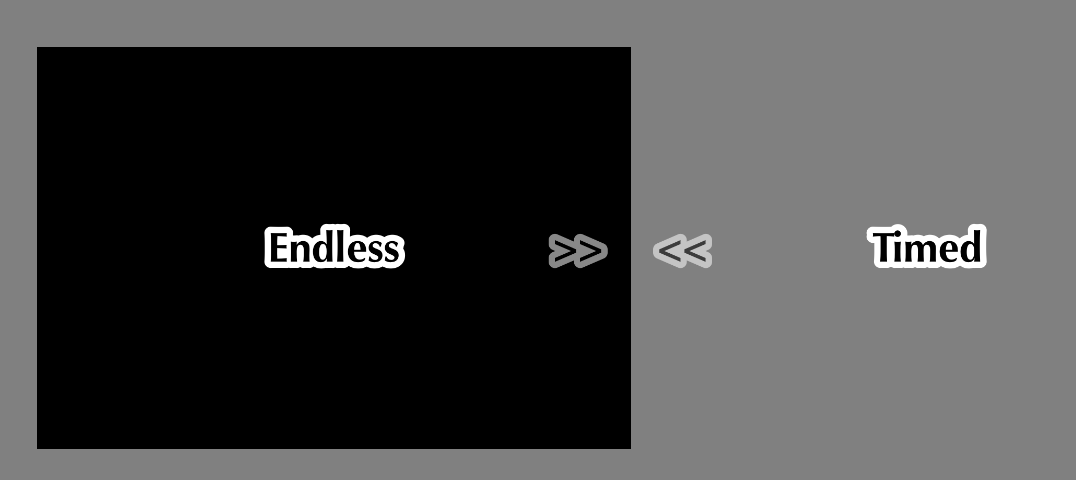
\includegraphics[width=250pt]{images/Chapter7/sv_result.png}
\end{figure}

Now we're ready to integrate this content node into a scroll view!

\begin{leftbar}
Add a scroll view to \textit{StartScene.ccb}:
\begin{enumerate}
  \item Open the \textit{StartScene.ccb} file
  \item Drag a \textit{Scroll View} from
the node library to the timeline of \textit{StartScene.ccb} and
drop it \textbf{below} (not on top of!) the \textit{background} node in the
timeline (so that the scroll view is rendered in front of the background image)
  
  \item Set the \textit{Position} to \textit{(0,0)}
  \item The scroll view shall cover the entire screen, so set the \textit{Content size
type} to \textit{Percent of parent container} for both \textit{Width} and
\textit{Height}
\item Set the \textit{Content Size} to \textit{(100, 100)}
\item Set up the scroll view specific settings in the
property inspector as follows:
\begin{figure}[H]
\centering
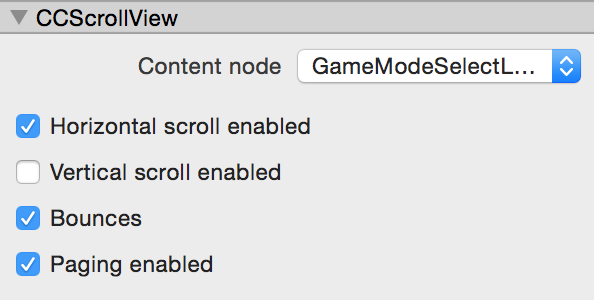
\includegraphics[width=250pt]{images/Chapter7/scrollview_settings.png}
\end{figure}
\end{enumerate}
\end{leftbar}

Let's discuss the scroll view settings briefly. The most important property is
the \textit{Content node} property. Here you can choose a \ccbfile{} that will
be displayed inside of the scroll view. We choose the
\inlinecode{GameModeSelectLayer.cbb} that we just created. We check
\textit{Horizontal scroll enabled} because the user shall only be able to scroll
left and right, not up or down. We discussed the option \textit{paging enabled}
briefly at the beginning of this section. With this setting activated the scroll
view will always snap to one of the game modes and will not allow the user to
stop scrolling in the middle of two game modes.

Great! At this point the set up of our start scene is almost complete.

\subsection{Finishing up the Game Mode Selection Scene}
As a last step we will implement the actual selection of one of the two game
modes. So far we have a scroll view that will allow users to switch between the
game modes but we don't have a mechanism to select one of the two and start a
game.

We will add a \textit{start} button to \textit{StartScene.ccb} that will
allow users to confirm a selected game mode and start the game. Once we have the button set up we will
add an animated transition from this game mode selection screen to the gameplay
scene. That transition will be triggered as soon as the player taps the start
button.

Let's start by adding a plain button. It is going to be positioned towards
the bottom of the screen, below the label that shows the selected game mode.

\begin{leftbar}
Add a start button to the game mode selection scene:
\begin{enumerate}
  \item Open \textit{StartScene.ccb} 
  \item Drag a \textit{Button} from the node library to
the stage, make sure it is below the \textit{background} node, just as the
scroll view we added earlier
  \item Set the \textit{Position Reference Corner} to \textit{Bottom-left}
  \item Set the \textit{Position Type} for \textit{X} to \textit{Percent of
  parent container}
  \item Set the \textit{X Position} to \textit{50} to center the node
  \item Set the \textit{Y Position} to \textit{80}
  \item Set the \textit{Preferred size} to \textit{100.0, 40.0}
  \item Set the \textit{Title} to \textit{Start!}
  \item Set the \textit{Font name} to \textit{Optima-Bold}
  \item Set the \textit{Font size} to \textit{17.00} 
\end{enumerate}
\end{leftbar}

Let's discuss some of the properties we just set up. As a short reminder - in
almost all cases we want to position UI elements relative to the screen corner
which they are closest to. This will result in the best behavior when the game
runs on different screen sizes. Therefore we choose the \textit{Bottom-Left}
corner as reference corner (technically we could also choose the
\textit{Bottom-Right}, since we are centering the button horizontally this
wouldn't make any difference).

Another interesting property is the \textit{Preferred Size}. Buttons
automatically resize to be large enough to enclose their content (in this case
the button text). If we want a button to appear larger than necessary we can set
the \textit{Preferred Size} property. In this example we make the button a
little bit larger than is required to fit the text \textit{Start!}.

We also need to set up some code connections. When the user taps the button we
want to start the transition. And there's another little feature that's
important. We only want to activate the \textit{Start!} button when the user has
selected one of the two game modes. If the user is currently scrolling between
two screen modes it shouldn't be possible to start the game. Otherwise it could
be pretty unclear to the user which game mode has been selected. We're going to
solve this issue by deactivating the button when a user is scrolling between
game modes.

\begin{leftbar}
Select the \textit{Start!} button and open the \textit{Code Connections}
tab. Set up a code connection with the \textit{Doc root var} and call it
\textit{playButton}. 
\end{leftbar}

We are going to use this code connection to activate and deactivate the start
button. Towards the beginning of this book we have discussed how we can connect
method calls to button taps (\ref{target_selector}). Now we are going to use
this functionality for the start button.

\begin{leftbar}
Set the \textit{selector} (method name) to \textit{playButtonPressed} and choose
the \textit{target} to be \textit{Document root}.
\end{leftbar}

As soon as the button is tapped the \inlinecode{playButtonPressed} method will
be called on the class of the root node. Right now the root node has no class set
up. Let's change that.

\begin{leftbar}
Select the root node (top most node in the timeline) of \textit{StartScene.ccb},
then open the code connections tab. Inside of the code connections tab set the
\textit{Custom class} to \textit{StartScene}.
\end{leftbar}

We'll need one more code connection for this scene - a connection for the
scroll view. Later, when we add some code to this scene you will see that we
need to connect to the scroll view to get informed when it
starts and stops scrolling. Whenever that happens we need to deactivate and
activate the start button accordingly.

\begin{leftbar}
Select the scroll view from the timeline and open the code connection tab. Set
up a code connection to \textit{Doc root var} and name that connection
\textit{scrollView}.
\end{leftbar}

Now we have all the code connections set up. Before we add some code to make
this scene work we will work through one last step in SpriteBuilder. We'll
create a nicely animated transition from the selection scene to the gameplay scene.

\subsection{Adding a Fancy Transition Animation}

Our transition will consist of two different components:
\begin{enumerate}
  \item The UI elements will move off the screen
  \item The background image will brighten up to full opacity
\end{enumerate}

Once these two steps are complete, the gameplay action will start.

Here's an illustration of what our transition will look like:
\begin{figure}[H]
		\centering
		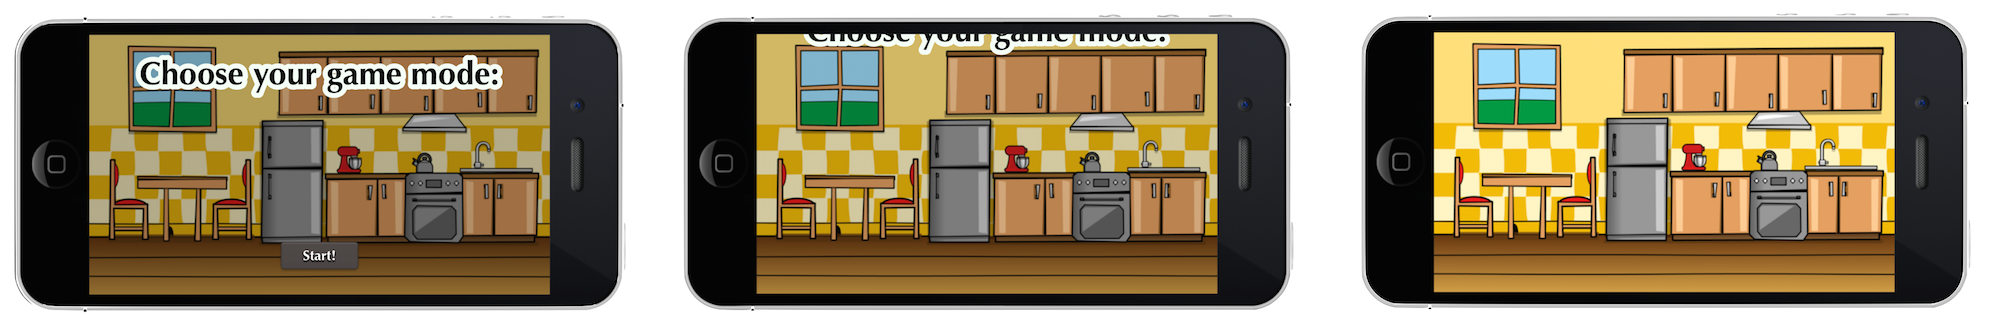
\includegraphics[width=0.85\linewidth]{images/Chapter7/gameplay_transition.png}
		\caption{By moving UI elements out of the screen and brightening the scene up
		we transition from the start scene to the gameplay scene}
\end{figure}

This transition is a nice example of how menus can be integrated into games
seamlessly. Using SpriteBuilder's timeline, creating this animation is pretty
straightforward. There are a bunch of steps involved, but none of them are
complicated. 

First, we'll need to create a new timeline. The default timeline runs
automatically as soon as the scene becomes visible. The animation we are about
to build, in contrast, shall only run when the user has selected a game mode.
Therefore we need to create new timeline which we can explicitly start playing
from code.

\begin{leftbar}
Create a new timeline for our transition animation:
\begin{figure}[H]
		\centering
		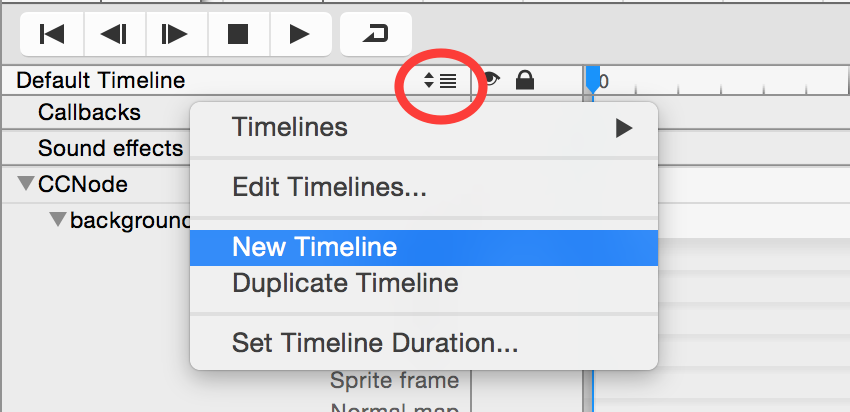
\includegraphics[width=200pt]{images/Chapter7/new_timeline.png}
\end{figure}
Next, rename the timeline. You can access the timeline editor through \SB{}'s
menu (\textit{Animation -> Edit Timelines\ldots}). Change the timeline name to
\textit{StartGameplay}.
\end{leftbar}
We want the transition to be pretty fast, so let's set the timeline duration to
1 second.
\begin{leftbar}
\begin{enumerate}
  \item Switch to the \textit{StartGameplay} timeline:
  \begin{figure}[H]
    \centering
    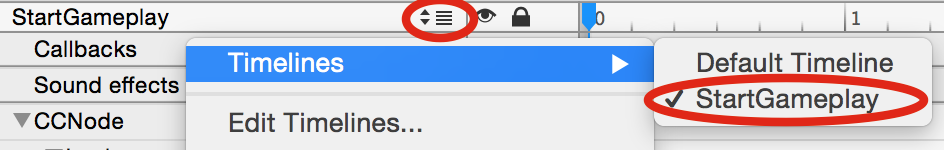
\includegraphics[width=200pt]{images/Chapter7/switch_timeline.png}
\end{figure}
  \item Set timeline duration to 1s. If you forgot how to change the timeline duration
you can skim back a few pages to figure \ref{fig: timeline_duration}
\end{enumerate}
\end{leftbar}
Next, we are going to set up keyframes for all of the UI elements that we want
to move off the screen. Additionally we will fade in the background sprite. Make
sure to follow the instructions exactly!
\begin{leftbar}
\begin{enumerate}
  \item Select the \textit{background} sprite
  \item Create an \textit{Opacity Keyframe} at 0 seconds and set the opacity
  value to \textit{0.7}
  \item Create a second \textit{Opacity Keyframe} at 1 second and set the
  opacity to \textit{1.0}
  \item Select the \textit{CCButton}
  \item Create a \textit{Position Keyframe} at 0 seconds, leave the position
  unchanged
  \item Create a second \textit{Position Keyframe} at 1 second and set the
  position to \textit{(50, -400)}
  \item Select the \textit{CCScrollView}
  \item Create a \textit{Position Keyframe} at 0 seconds, leave the position
  unchanged
  \item Create a second \textit{Position Keyframe} at 1 second and set the
  position to \textit{(0, -400)} 
  \item Select the \textit{CCLabelTTF}
  \item Create a \textit{Position Keyframe} at 0 seconds, leave the position
  unchanged
  \item Create a second \textit{Position Keyframe} at 1 second and set the
  position to \textit{(50, -50)}  
\end{enumerate}
\end{leftbar}
Great! If you want you can test the animation with the \SB{} timeline playback
feature.

There's one last step left in \SB{} before we move to \xcode{} and implement the
actual transition between start scene and gameplay. As soon as the animation
completes, that means all UI elements have moved off the screen and the
background is brightened up completely, we want to switch to the gameplay scene.
Switching scenes has to be implemented in code. This means that we need a
callback in code that gets triggered as soon as this animation completes.

\SB{} and \cocos{} provide three different ways to implement this:
\begin{itemize}
  \item Provide a completion block to the animation manager of a scene. This
  completion block will be called whenever a timeline animation completes
  \item Implement a delegate method that gets called by the animation manager
  when a timeline animation completes
  \item Set up a callback method within a \SB{} timeline animation
\end{itemize}

For this section I want to go with the last option. The ability to call methods
as part of timeline animations can be useful in many situations, so I want to
use it as early as possible!

\begin{leftbar}
To add a callback method to a timeline animation you need to \textit{Option-Key
+ Click} into the \textit{Callbacks} line of the timeline editor:

\begin{figure}[H]
		\centering
		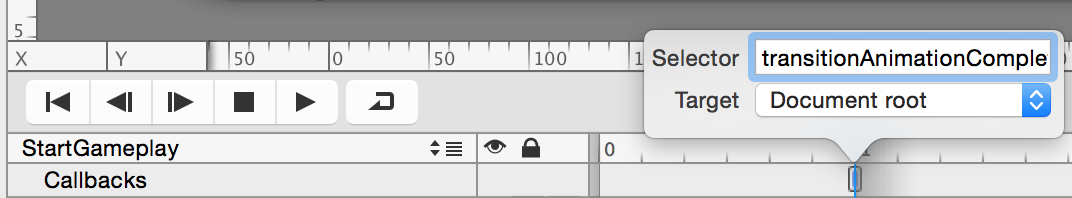
\includegraphics[width=300pt]{images/Chapter7/timeline_callback.png}
\end{figure}
Place that callback at 1 second. You can also choose the \textit{target} and
\textit{selector} for this callback. Select \textit{Document root} as target and
\textit{transitionAnimationComplete} as selector.
\end{leftbar}

Great! This was quite a lot of work, but now we have a game mode selection
scene (including a scroll view) and a great transition into the gameplay scene.
Now it's time to switch back to code!

\subsection{Implementing the Game Mode Selection}

\begin{leftbar}
Publish the \SB{} project and switch to the \xcode{} project.
\end{leftbar}

The first change we need to make to the \xcode{} project is to set up which
scene gets presented when our game starts\index{Start Scene}. By default it's
the \textit{MainScene}. However, we have created a new \textit{StartScene} and want
that one to be the first scene of the game.

We can change this setting in the \textit{AppDelegate} of the project. 
\begin{leftbar}
Open \textit{AppDelegate.m} in \textit{Source/Platforms/iOS/}:
\begin{figure}[H]
		\centering
		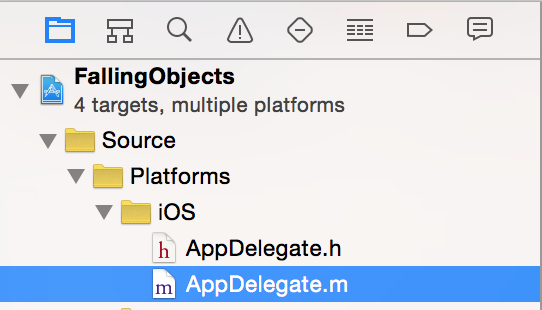
\includegraphics[width=200pt]{images/Chapter7/app_delegate.png}
\end{figure}
\end{leftbar}

The \inlinecode{AppDelegate} of \cocos{} is written in Objective-C. If you don't
know Objective-C, don't worry, the change we need to make is trivial.

When a \cocos{} game starts, the \inlinecode{startScene} method of the
\inlinecode{AppDelegate} gets called. That method is responsible for loading and
returning the start scene of the game. Let's modify it to load
\inlinecode{StartScene} instead of \inlinecode{MainScene}.

\begin{leftbar}
Modify the \inlinecode{startScene} method of \textit{AppDelegate.m} to look as
following:
\begin{lstlisting}
- (CCScene*) startScene
{
    return [CCBReader loadAsScene:@"StartScene"];
}
\end{lstlisting}
\end{leftbar}
Great! Now our new start scene will be presented when our game starts. Note
that the game won't run at this point. We need to create the
\inlinecode{StartScene} class. We're already referencing this class from the
\SB{} project, but we haven't created it yet.

\begin{leftbar}
Create a new Swift file. Call it \inlinecode{StartScene}. Set up the basic
\inlinecode{StartScene} class like this:
\begin{lstlisting}
class StartScene: CCNode {
  
  weak var scrollView: CCScrollView!
  weak var playButton: CCButton!
  var selectedGameMode: MainScene.GameModeSelection = .Endless
  
}
\end{lstlisting}
\end{leftbar}
The first two variables are necessary for the code connections that we set up
in our \SB{} project. The third variable stores which game mode the player has
currently selected. Since the game mode is a choice between multiple options an
enum is a great way to model this. The enum referenced here
(\inlinecode{MainScene.GameModeSelection}) does not exist yet. We need to add it to the
\inlinecode{MainScene} class.

\begin{leftbar}
Open \textit{MainScene.swift} and add the following lines:
\begin{lstlisting}
var selectedGameMode: GameModeSelection?
  
enum GameModeSelection: Int {
  case Endless
  case Timed
}
\end{lstlisting}
\end{leftbar}
The first line is a property that stores the game mode of the current game.
Later we will use that property to apply different rules to the gameplay and
display different score information based on the game mode that player picker.
The information on which game mode the player has picker will be handed to us by
the \inlinecode{StartScene}.

We've also added an enum definition. The \inlinecode{GameModeSelection} enum has two
different states, one for each game mode. For now we will only implement an
endless and a timed game mode. As we've done earlier, we are associating
\textit{raw values} with this enum by adding the \inlinecode{Int} type after the
enum name. This means that the \inlinecode{Endless} value corresponds to 0 and
the \inlinecode{Timed} value corresponds to 1.

Now we can switch back to working on our new start scene. There are three
features we need to implement in \textit{StartScene.swift}. We need to keep
track of the movement of the scroll view. When the user scrolls to one of the
two pages of the scroll view, we need to remember which game mode has been
chosen. Further, as discussed earlier, we need to deactivate the \textit{Start!}
button while the user scrolls. Finally, we need to trigger a transition to the
gameplay scene (\inlinecode{MainScene}) as soon as a user taps the start button.
As part of that transition we need to inform \inlinecode{MainScene} which game
mode was selected. Let's start with the scroll view related code.

\subsubsection{Implementing a Scroll View Delegate}\index{User
Interface!CCScrollView!Delegate}
If you have written code for the iOS platform before, you are very familiar with
the principle of delegation. However, this book does not necessarily require
previous iOS app development knowledge.

If you haven't heard of delegation before, Apple has a great introduction in
their developer guide:
\url{https://developer.apple.com/library/ios/documentation/General/Conceptual/DevPedia-CocoaCore/Delegation.html}.

The \inlinecode{CCScrollView} in \cocos{} also uses the delegate pattern. This
is what the (Objective-C) protocol looks like:
\begin{lstlisting}
@protocol CCScrollViewDelegate <NSObject>

@optional
- (void)scrollViewDidScroll:(CCScrollView *)scrollView;
- (void)scrollViewWillBeginDragging:(CCScrollView *)scrollView;
- (void)scrollViewDidEndDragging:(CCScrollView * )scrollView willDecelerate:(BOOL)decelerate;
- (void)scrollViewWillBeginDecelerating:(CCScrollView *)scrollView;
- (void)scrollViewDidEndDecelerating:(CCScrollView *)scrollView;

@end
\end{lstlisting}

There are a total of five methods that we can implement. The
\inlinecode{optional} keyword marks a section of the protocol in which all
listed methods are not required to be implemented. In this specific protocol \textit{all} methods are optional. 

We want to be informed when the scroll view starts and ends scrolling. There are
two methods that get called in these cases:
\inlinecode{scrollViewWillBeginDragging} and
\inlinecode{scrollViewDidEndDecelerating}. Let's become the delegate of our
scroll view and implement these methods.

The first step is setting ourselves up as the delegate of the scroll view. We
can set ourselves as the delegate as soon as the scene is entirely loaded (when
\inlinecode{didLoadFromCCB} is called). 
\begin{leftbar}
Add the following implementation of \inlinecode{didLoadFromCCB} to
\inlinecode{StartScene}:
\begin{lstlisting}
func didLoadFromCCB() {
  scrollView.delegate = self
}
\end{lstlisting}
\end{leftbar}
Now the scroll view knows about us and will call all the methods of the
\inlinecode{CCScrollViewDelegate} protocol that we implement.

Next, we need to add the protocol implementation. In Swift it is common to
implement protocols in class extensions. Class extensions allow us to add functionality to
a class outside of its original definition. Moving all protocol
implementations into separate class extensions is a nice way of keeping our code
organized. 

The implementation of our two protocol methods is pretty simple. When the user
starts scrolling we deactivate the start button. When the user ends scrolling,
we activate the start button and remember the selected game mode.
\begin{leftbar}
Add the following protocol implementation to \filemention{StartScene.swift}. It
is \textbf{important} that the class extension is \textbf{not} part of the
class, but placed after the closing curly brackets of the class definition:
\begin{lstlisting}
class StartScene: CCNode {
  ...  
}

extension StartScene: CCScrollViewDelegate {
  
  func scrollViewWillBeginDragging(scrollView: CCScrollView) {
    playButton.enabled = false
  }
  
  func scrollViewDidEndDecelerating(scrollView: CCScrollView) {
    playButton.enabled = true
    selectedGameMode = MainScene.GameModeSelection(rawValue: Int(scrollView.horizontalPage))!
  }
  
}
\end{lstlisting}
\end{leftbar}
Activating and deactivating the button is very simple; \inlinecode{CCButton}
provides a property for it. Choosing the game mode based on the selected scroll
view page is similarly straightforward. \inlinecode{CCScrollView} provides a
\inlinecode{horizontalPage} property that allows use to read which page the user
has currently scrolled to. We use that value to select the according game mode.
In order to create an enum value from a number we need to use the
\inlinecode{rawValue:} initializer (remember that 0 corresponds to the endless
game mode and 1 to the timed game mode).

Our work with the scroll view is completed. Next, let's implement the callback
method for the button interaction. As soon as the play button is tapped we want
to play the transition animation that we created in \SB{}. Additionally, we
should deactivate the scroll view. That way users cannot modify the selected
game mode while the scene is in transition.

\begin{leftbar}
Implement the \inlinecode{playButtonPressed} method that we've set up in \SB{}
inside of \inlinecode{StartScene}. This should be implemented as part of the
core class, not of the extension:
\begin{lstlisting}
  func playButtonPressed() {
    scrollView.userInteractionEnabled = false
    animationManager.runAnimationsForSequenceNamed("StartGameplay")
  }
\end{lstlisting}
\end{leftbar}
First, we deactivate user interaction on the scroll view. Whichever game mode
has been selected by the user before hitting the play button will stay selected
throughout the animation. Then we run the actual animation. Remember that all
timelines created in \SB{} can be referenced in code by using their name.

Now there's a last method left to be implemented. We have added a callback to
the timeline animation that gets called when the transition animation is
completed. In the implementation of that method we should perform the actual
scene transition, which means replacing the \inlinecode{StartScene} with the
\inlinecode{MainScene}. The animation that we are running only moves the UI
elements off the screen. However, as you might remember transition between
scenes can only be implemented in code.

Transitions between scenes can also be animated. For the
transition from the start scene to the gameplay scene we will use a cross fade
transition. Add the end of our timeline animation the start scene is entirely
empty. Then we use a cross fade animation to transition to the gameplay scene
where the pot will be displayed. The cross fade animation will make the pot
appear slowly before the actual game starts.

\begin{leftbar}
Add the following implementation for the timeline callback, that we've set up in
\SB{}, to \inlinecode{MainScene}:
\begin{lstlisting}
func transitionAnimationComplete() {
  let scene = CCBReader.loadAsScene("MainScene")
  let gameplay = scene.children[0] as! MainScene
  gameplay.selectedGameMode = selectedGameMode
  let transition = CCTransition(crossFadeWithDuration: 0.7)
  CCDirector.sharedDirector().replaceScene(scene, withTransition: transition)
}
\end{lstlisting}
\end{leftbar}
This method gets called as soon as the transition animation ends. Within it we
perform some scene transition code with which you should be familiar from our
very first \SB{} project. That code hides the \inlinecode{StartScene} and
presents the \inlinecode{MainScene}.

Great! Now our game mode selection screen is complete; including an awesome
transition to the gameplay scene. You can run the project and try it out.

The next big step for our project is implementing the two different game modes.
While implementing the game modes you will learn how to build modular and
extensible code! 

We will start off by creating two different UIs for the two game
modes. 

In the endless game mode the player will loose health for dropping items
or collecting incorrect items and will gain health for collecting correct items. For the endless mode we need to
display a health bar. 

In the timed mode the player will have a hard time limit. For that mode
we need to display a counter that shows the remaining time and a score label.

\section{Implementing Multiple Game Modes}
Let's get started on building the two different game modes. 

We're going to start with setting up the UI in for each game mode in \SB{}. Then
we will come up with a way to implement the two game modes without duplicating
code - this is a great use case for exploring some potential design patterns for
game development.

\subsection{Adding UIs for Different Game Modes}
Open your \SB{} project. We're going to create two separate \ccbfile{}s, one for
the UI elements of each game mode.

\subsubsection{UI for the Timed Game Mode}
\begin{leftbar}
\begin{enumerate}
  \item Create a new \ccbfile{} of type \textit{Layer} and name it
  \textit{TimedModeUI}
  \item Select the root node of the new \ccbfile{} and change the
  \textit{Content size type} to be \textit{percentage of parent container} for
  both, width and height
  \item Set the \textit{Content Size} to \textit{(100, 100)}
\end{enumerate}
\end{leftbar}

We will place all UI elements relative to the edges of the screen. That way the
UI will look good on any given screen size. That's why we want the root node to
take 100\% the size of its parent container. If we instead would use a fixed
size for this layer our UI would not respond to multiple screen sizes.

The UI for the timed game mode is not too complicated, it consists of two
separate labels. We want the style of these labels to be consistent with the
labels that we used on the start scene. The easiest way to do accomplish this is
to actually copy the label in \SB{}.

\begin{leftbar}
\begin{enumerate}
  \item Open \filemention{StartScene.ccb}
  \item Select the \textit{CCLabelTTF} from the
timeline
\item Now select \textit{Edit -> Copy} from the \SB{} menu (or use the
shortkey: \textit{CMD+C})
\item Next, open \filemention{TimedModeUI.ccb}
\item Select \textit{Edit -> Paste} from
the \SB{} menu (or use: \textit{CMD+V}).
\end{enumerate} 
\end{leftbar}

Now you should have an exact copy of the start scene label in your new
\ccbfile{}. We'll make a small tweak to this label and lay it out
correctly.

\begin{leftbar}
Apply the following changes to the label:
\begin{enumerate}
  \item Select the \textit{Position Reference Corner} to be the top left corner
  \item Change the \textit{Position Type} for \textit{X} to be \textit{in
  Points}
  \item Change the position to \textit{(20,20)}
  \item Change the anchor point to \textit{(0.0, 1.0)}
  \item Change the label text to \textit{Time: 0}
  \item Change the font size to \textit{30}
  \item Set up a code connection to the \textbf{Owner var} (not the \textit{Doc
  root var}; this is very important!) and name it \textit{timeLabel}
\end{enumerate}
\end{leftbar}

Now the label should be nicely positioned in the top left corner! 

This is the first time we are using a variable which is assigend to the
\textbf{Owner var}. We will not be creating a custom class for this \ccbfile{},
since it doesn't have any specific behavior that we need to implement. 

Instead we will later assign the code connections to the classes that
contain the actual gameplay logic. The \inlinecode{MainScene} instance will
become the owner of this \ccbfile{} which means it will have access to all
\textit{Owner vars}.

That's why it's important to set up the code connection with the \textit{Owner var} instead of the \textit{Doc root var}.

Next, let's create the points label. Since it will look almost identical to the
time label we should save some time and just copy and modify the label again
instead of starting with a new label from scratch. Note however, that you should
be careful when using this approach. When you copy a node all of its
properties are copied along with it (including code connections). If you aren't
careful you might end up with hard to debug issues (e.g two nodes attempt to use
the same code connection variable).

\begin{leftbar}
Copy the time label that you just created it and paste it. Change the pasted
label as following:
\begin{enumerate}
  \item Select the \textit{Position Reference Corner} to be the top right corner
  \item Change the \textit{Anchor point} to \textit{(1.0, 1.0)}
  \item Change the \textit{label text} to \textit{Points: 0}
  \item Set the \textit{Position} to \textit{(20, 20)}
  \item Set up a code connection to the \textbf{Owner var} and name it \textit{pointsLabel}
\end{enumerate}
\end{leftbar}

Great! The UI for the timed game mode is completed. It should look as following:

\begin{figure}[H]
    \centering
    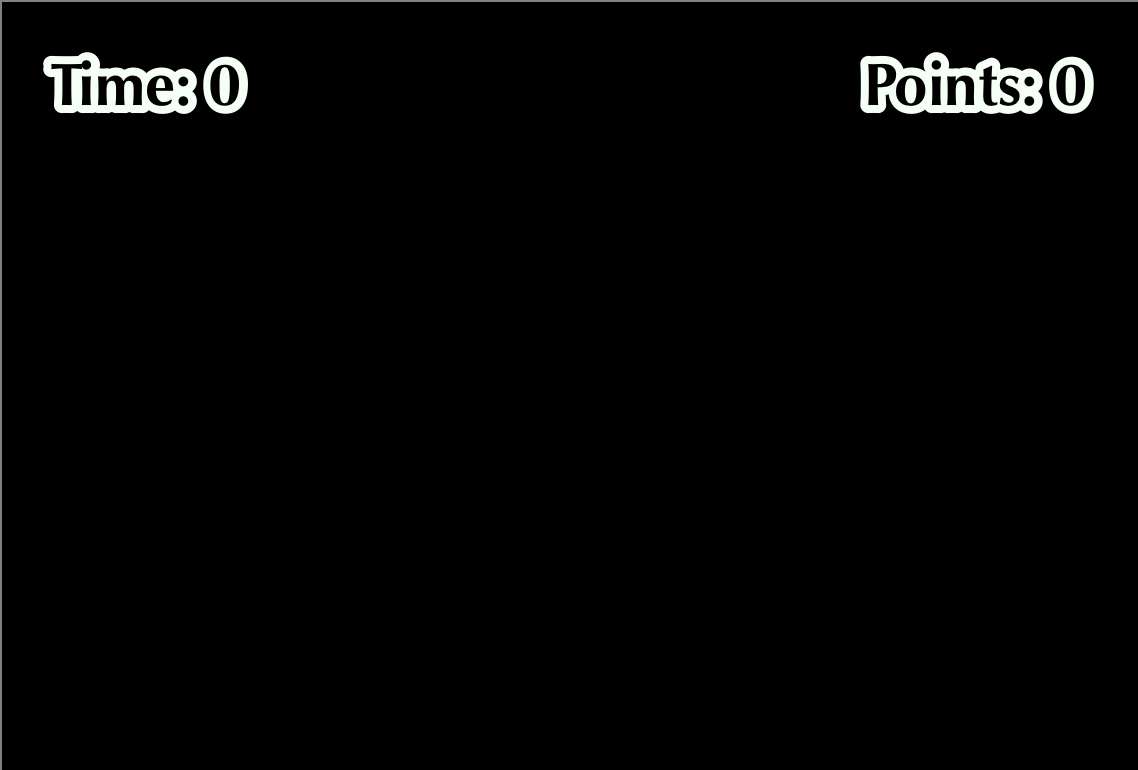
\includegraphics[width=0.5\linewidth]{images/Chapter7/timed_mode_ui.png}
\end{figure}

\subsubsection{UI for the Endless Game Mode}
Now, let's create the  UI for the endless game mode which will contain a health
bar. We'll start of by creating a new \ccbfile{}.

\begin{leftbar}
Set up the \ccbfile{} for the endless game mode UI:
\begin{enumerate}
  \item Create a new \ccbfile{} of type \textit{Layer} and name it
\textit{EndlessModeUI}
\item Select the root node of the new \ccbfile{} and change
the \textit{Content size type} to be \textit{Percent of parent container} for
both, width and height
\item Set the \textit{Content Size} to \textit{(100, 100)}
\end{enumerate}
\end{leftbar}
Next, let's add a label that displays the amount of seconds a player has
survived. Once again we can copy the existing label from the
\filemention{TimeModeUI.ccb} file since we want both labels to look identical.
\begin{leftbar}

Open \filemention{TimeModeUI.ccb} and copy the label in the \textbf{top left
corner}. Then open \filemention{EndlessModeUI.ccb} and paste the label. Select
the pasted label and modify it as following:
\begin{enumerate}
  \item Change the label text to \textit{Survived: 0}
  \item Set up a code connection to the \textbf{Owner var} and name it \textit{survivedLabel}
\end{enumerate}
\end{leftbar}

Besides this label we will also need to display a health bar in the endless game
mode. The easiest way to implement a health bar in \cocos{} is taking a plain
\inlinecode{CCColorNode} and scaling it depending on the current health level
of the player.

\begin{leftbar}
Add the health bar to \textit{EndlessModeUI.ccb}:
\begin{enumerate}
  \item Drag a \textit{Color Node} from the node library to the stage
  \item Select the \textit{Position Reference Corner} to be the \textit{top
  right corner}
  \item Change the \textit{Position} to \textit{(20,20)}
  \item Change the \textit{Anchor point} to \textit{(1.0, 1.0)}
  \item Chante the \textit{Content size} to \textit{(150, 40)}
  \item Change the node color to \textit{green} (or pick any other color you
  enjoy)
  \item Set up a code connection to the \textbf{Owner var} and name it \textit{healthBar}
\end{enumerate}
\end{leftbar}

Now the UI for the endless mode should look like this:

\begin{figure}[H]
    \centering
    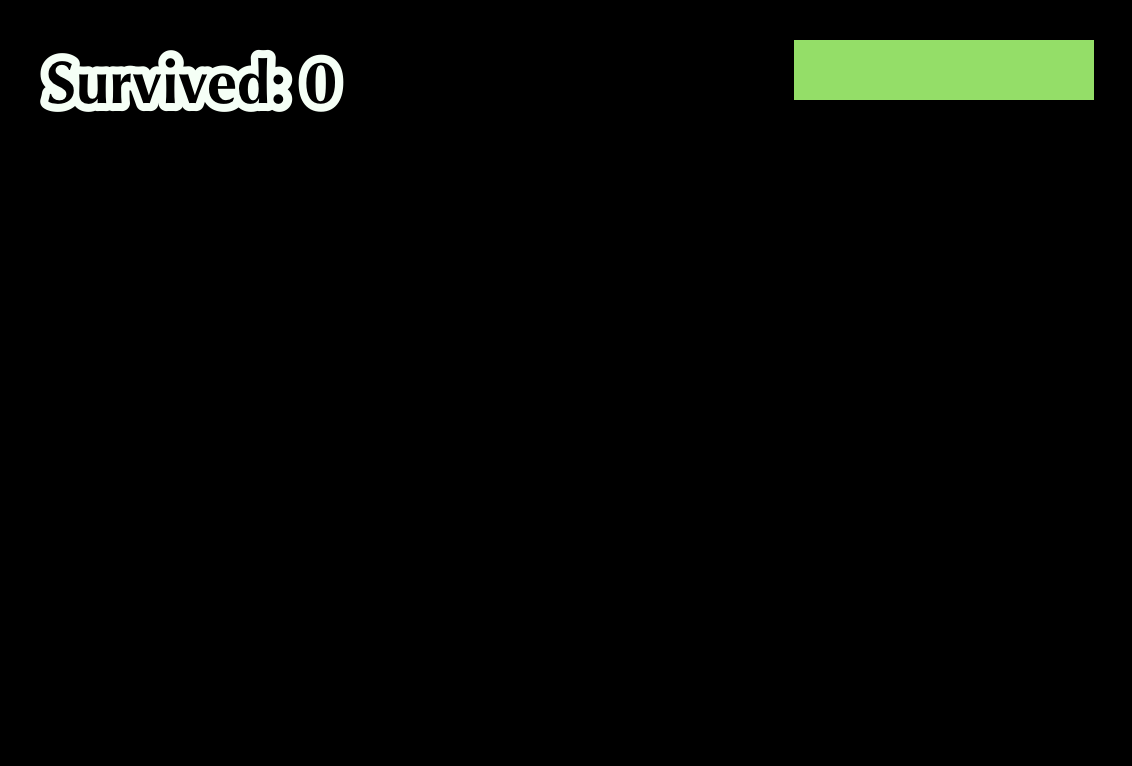
\includegraphics[width=0.5\linewidth]{images/Chapter7/endless_mode_ui.png}
\end{figure}

We're done with the UI setup. To make these score displays actually show up as
part of the game, we'll now move to implementing the two game modes!

\subsection{Implement Game Logic for Different Modes}
We need to change multiple parts of our game to support two different game
modes. Depending on which game mode a player selects, we want to display a
different score board and also implement a different set of rules.

We want to implement a design that allows us to add many more game modes in
future - without convoluting the code base.

Before we dive into coding, let's try to figure out what we'll need to
implement:
\begin{itemize}
  \item When we start a game, the \inlinecode{MainScene} class needs to know
  which game mode a user has selected
  \item \inlinecode{MainScene} shouldn't know
  anything about the rules of the selected game mode. That way we could create
  additional game modes in future without increasing the complexity of
  \inlinecode{MainScene}
  \item Every game mode should know about its rules (when does a player earn /
  loose points, when does a game end)
  \item Every game mode should know which score board entries it has and it
  should be responsible for updating them based on the current state of the game
\end{itemize}

We should try to come up with a solution that lets us add more game modes as
easily as possible. One modular way of implementing this is setting up different
game modes as individual classes. These classes can be referenced by the
\inlinecode{MainScene} class. In this scenario, the \inlinecode{MainScene} class
remains responsible for the core of the game, it spawns falling objects (though,
even this could be moved into the gameplay classes eventually) and lets them
fall to the ground. It handles collision detection and determines if an object
was caught or dropped.

The consequences of catching or dropping objects however, are not implemented in
the \inlinecode{Gameplay} class itself. Instead, they are implemented by the
game modes. This means that the \inlinecode{Gameplay} class needs to inform the
game mode when a significant event occurs. The game mode itself can then decide
how this event impacts the gameplay.

Here's a diagram that illustrates our solution:

\begin{figure}[H]
    \centering
    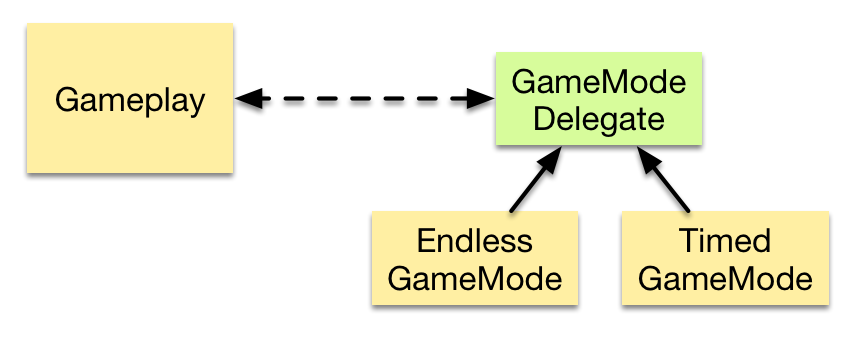
\includegraphics[width=0.5\linewidth]{images/Chapter7/gameplay_design.png}
\end{figure} 

We'll create a \inlinecode{GameMode} protocol that defines the
communication between \inlinecode{MainScene} and the different game modes. Each
game mode will implement the \inlinecode{GameMode} protocol.

\subsubsection{Defining a Protocol for Game Modes}
Let's start implementing this design. The first step is defining a protocol
that can be implemented by all game modes. In the diagram above I've highlighted
the protocol in green.

As discussed, there are three events that we are interested in; all of them
should be part of our protocol.
\begin{leftbar}
Create a new Swift file in \xcode{} and call it
\filemention{GameMode.swift}.
Then add the following protocol definition to it:
\begin{lstlisting}
typealias GameOver = Bool

protocol GameMode: class {
  var userInterface: CCNode! { get }

  func gameplay(mainScene:MainScene, droppedFallingObject:FallingObject)
  func gameplay(mainScene:MainScene, caughtFallingObject:FallingObject)
  func gameplayStep(mainScene:MainScene, delta: CCTime) -> GameOver
}
\end{lstlisting}
\end{leftbar}
Note that I have omitted the source code documentation of this protocol for the
sake of brevity. 

The protocol we've just defined will be implemented by
multiple classes, it's important to document its methods and properties for developers that want
to add game modes in future. You can take a look at the source code for
this protocol on
GitHub
(\url{https://github.com/SpriteBuilder-Book/Code/blob/master/Chapter7/FallingObjects.spritebuilder/GameMode.swift}) to read the documentation.

\begin{details}[Source code
documentation in Swift] Many details about source code documentation in Swift are still up in the air.
NSHipster provides a great article that describes the currently supported
documentation style: \url{http://nshipster.com/swift-documentation/}.
\end{details}

Let's discuss this protocol in detail. The first interesting aspect is a
\inlinecode{typealias} statement before the protocol declaration. The
\inlinecode{typealias} keyword in Swift allows us to give a type a new alias
name. In this case we are creating a new type called \inlinecode{GameOver} which
is actually just a \textit{Bool}. Using \inlinecode{typealias} is a nice way
of better capturing the semantics of a type. A method that returns a
type of \inlinecode{GameOver} is easier to understand than a method returning a
plain \inlinecode{Bool}.

The second thing to note is that we
have defined the protocol as a \textit{class-only} protocol. We can do that by
adding the \inlinecode{class} keyword to the protocol's inheritance list. Later
you'll see that any type that implements \inlinecode{GameMode} is
required to be a reference type, because we need to pass references to it to the
\cocos{} framework. 

We start our protocol by defining a property: \inlinecode{userInterface}. This
property shall provide access to the game mode's user interface. The
\inlinecode{MainScene} class can use this property to access the UI for the
currently active game mode.
We only expose as a getter as part of the protocol, the UI cannot be assigned
from outside of the game mode class. Each game mode creates its own UI and is
responsible for holding on to it.

Next, we define two methods that get called when objects get dropped or caught.
Both methods receive a reference to the \inlinecode{MainScene}. This is pretty
common when using the delegate pattern. Theoretically a game mode instance
could be the delegate of multiple \inlinecode{MainScene} instances. By passing
the \inlinecode{MainScene} in which the event occurred to the delegate the
delegate gets the chance to respond differently depending which instance has
called the method. It's good to conform to that convention - however we won't
sign up as the delegate of multiple \inlinecode{MainScene} instances.

The second parameter sent to both methods is the object which has been caught or dropped. The class implementing
the \inlinecode{GameMode} can use this information to determine whether
points should be added or subtracted.

The last method(\inlinecode{gameplayStep:}) fulfills two purposes. Firstly, it
allows game modes to hook into the update method of \inlinecode{MainScene}. That
is necessary for any time based actions, e.g. capturing the total time that
has passed since the beginning of the game. The second purpose is fulfilled by
the \inlinecode{GameOver} return value. The return value allows the game mode to
tell the \inlinecode{MainScene} that the game is over. All game modes will use
this method to implement the game over condition.

Now that our protocol is defined we can implement the two game modes. 

\subsubsection{Implementing the Timed Game Mode}
Let's start by implementing the timed game mode. Since we thought about the
software design upfront and even defined a protocol for game modes, the
implementation itself is not too complicated.

\begin{leftbar}
Create a new Swift file and name it \filemention{TimedGameMode}. Add the
following class definition to the new file:
\begin{lstlisting}
@objc(TimedGameMode)
class TimedGameMode: GameMode {
  var timeLabel: CCLabelTTF!
  var pointsLabel: CCLabelTTF!
}
\end{lstlisting}
\end{leftbar}
There's a lot going on in these few lines. Firstly, we need the
\inlinecode{@objc} annotation to make this class visible to \cocos{}. \cocos{}
is written in Objective-C and can only see classes that are subclasses of
\inlinecode{NSObject} or that have the \inlinecode{@objc} annotation. So far all
of our classes have been subclasses of \cocos{} classes, and all of them in turn
are derived from \inlinecode{NSObject}, therefore this annotation wasn't
necessary. The \inlinecode{TimedGameMode} class is our first class that is not a
subclass of an Objective-C class.

In the second line we declare that our class conforms to the
\inlinecode{GameMode} protocol. We also declare two properties
for the code connections that we set up in the \ccbfile{} for the timed game
mode. We have access to two different labels, one displays the player's
points the other one displays the time that's left.

We'll need a whole set of additional variables. We need a
\inlinecode{userInterface} variable to conform to the
\inlinecode{GameMode} protocol. We also need variables to store the amount of
points the player has scored and the time that is left in the current game.

\begin{leftbar}
Add the following properties and property observers to the
\inlinecode{TimedGameMode} class:
\begin{lstlisting}
let minPoints = 0
let minTime = 0.0

private(set) var userInterface: CCNode!

private var time: CCTime = 10 {
  didSet {
    updateTimeDisplay(time)
  }
}

private var points: Int = 0 {
  didSet {
    updatePointsDisplay(points)
  }
}
\end{lstlisting}
\end{leftbar}
The first two constants are used to define the bottom line for time and points
in this game mode. In almost all cases using constants should be preferred over
using number literals directly in code. By defining constants our intentions are
obvious to other developers and we can update the values in one place.

Further, we add the \inlinecode{userInterface} variable. This variable will
store the loaded \ccbfile{} that belongs to the timed game mode. It is also
required to conform with the \inlinecode{GameMode} protocol.

Next, we declare and define the \inlinecode{time} property that stores the time
that is left during the current game. For testing purposes our games only last 10 seconds. We
also add a property observer. When the time value changes we call the (yet to
be implemented) \inlinecode{updateTimeDisplay:} method, that method updates the
label that displays the leftover time.

We essentially do the same for the \inlinecode{points} property.

Next, let's implement the two helper methods that update the time and point
labels.
\begin{leftbar}
Add the following two methods to \inlinecode{TimedGameMode}:
\begin{lstlisting}
func updatePointsDisplay(points: Int) {
  pointsLabel.string = "Points: \(points)"
}

func updateTimeDisplay(time: CCTime) {
  timeLabel.string = "Time: \(Int(time))"
}
\end{lstlisting}
\end{leftbar}
These methods are very simple. We only warp this code into separate methods
because we need the functionality in multiple places, as you'll see shortly.

Next, before we implement the methods defined in our protocol, let's tackle the
initializer of this class. The main task the initializer needs to perform is
loading the game mode's UI from a \ccbfile{}.
\begin{leftbar}
Add the following initializer:
\begin{lstlisting}
init() {
  userInterface = CCBReader.load("TimedModeUI", owner:self)
  updatePointsDisplay(points)
  updateTimeDisplay(time)
}
\end{lstlisting}
\end{leftbar}
In the first line we load the \filemention{TimedModeUI} \ccbfile{}. We store the
loaded node hierarchy in the \inlinecode{userInterface} property, that way it
can be accessed by \inlinecode{MainScene}.
We also call our two label helper methods, so that the labels display the
correct initial values for time and points.

Now we can move on to the core of this class: the methods that are required by
the \inlinecode{GameMode} protocol.

Let's start with the \inlinecode{gameplay(mainScene:,
droppedFallingObject:)} method. At this point it's time to make some
decisions on the rules of the timed game mode. 

I suggest that we subtract 1 point when the player
drops an object that should be caught. Because we don't want to be too mean we
set the lowest possible score to 0.

\begin{leftbar}
Add the following method to \inlinecode{TimedGameMode}:
\begin{lstlisting}
func gameplay(mainScene:MainScene, droppedFallingObject:FallingObject) {
  if (droppedFallingObject.type == .Good) {
    points = max(points - 1, minPoints)
  }
}
\end{lstlisting}
\end{leftbar}
If the object that has been dropped is a \inlinecode{.Good} object, we subtract
one point. Using Swift's \inlinecode{max} function we make sure that the total
score never drops below \inlinecode{minPoints}, which we have defined as 0.

If a \inlinecode{.Bad} object drops the score is not influenced. Therefore we
don't need to cover this case here.

Next, we'll implement the method that gets called when objects are caught.
Once again time to decide on some rules. I propose to add a point when a good
object is caught and subtract a point when a bad object is caught. You can
obviously feel free to use different values!

\begin{leftbar}
Add the method for caught objects to \inlinecode{TimedGameMode}:
\begin{lstlisting}
func gameplay(mainScene:MainScene, caughtFallingObject:FallingObject) {
  switch (caughtFallingObject.type) {
  case .Bad:
    points = max(points - 1, minPoints)
  case .Good:
    points += 1
  }
}
\end{lstlisting}
\end{leftbar}
Since we are checking for multiple possible values of an enum using a switch
statement results in nicely readable code. Besides the switch statement the
implementation is pretty straightforward.

Now there's only one last method to implement:
\inlinecode{gameplayStep(mainScene:, delta:)} We need to do two things in the
implementation of this method:
\begin{enumerate}
  \item Subtract the passed time (\inlinecode{delta}) from the remaining game
  time
  \item Check if the remaining time reached the minimum time (0.0) and return
  \inlinecode{true} if that's the case
\end{enumerate}
\begin{leftbar}
Add the following implementation of the step method to
\inlinecode{TimedGameMode}:
\begin{lstlisting}
func gameplayStep(mainScene: MainScene, delta: CCTime) -> GameOver {
  time -= delta
  return !(time > minTime)
}
\end{lstlisting}
\end{leftbar}
First, we subtract \inlinecode{delta} from the remaining game time. Next, we
check if the total time is over or not and return a \inlinecode{GameOver} value
based on that.

Congratulations! We have fully implemented our first game mode. Now, let's
implement the endless game mode.

\subsubsection{Implementing the Endless Game Mode}
The procedure for implementing the endless game mode will be very similar to the
timed one: Setting up code connections, implementing game mode rules and
updating the scoreboard.

Let's start with setting up the basic class and code connections.
\begin{leftbar}
Create a new Swift file in \xcode{} and name it \textit{EndlessGameMode}. Then
add the following class definition and properties:
\begin{lstlisting}
@objc(EndlessGameMode)
class EndlessGameMode: GameMode {
  var healthBar: CCNode!
  var survivedLabel: CCLabelTTF!
}
\end{lstlisting}
\end{leftbar}
As I said, this is pretty similar to the timed game mode. We need the
\inlinecode{@objc} annotation because this class does not inherit from an
Objective-C class. We declare two properties for the two UI elements in the
\filemention{EndlessModeUI} \ccbfile{}.

In the endless game mode we will have two game parameters that we want to keep
track off: the current \textit{health} of the player and the
\textit{survivalTime} of the current game. In the endless game mode the player
has the goal of surviving as long as possible. Instead of gaining points for
catching objects the player regains some health. Whenever the player catches an
incorrect object or drops a good object she looses health. We'll need properties
to keep track of these values.

Additionally we'll need a property that stores the UI node to conform with the
\inlinecode{GameMode} protocol.

\begin{leftbar}
Add the following properties and property observers to
\inlinecode{EndlessGameMode}:
\begin{lstlisting}
private(set) var userInterface: CCNode!
private let minHealth = 0
private let maxHealth = 10

private var health:Int = 10 {
  didSet {
    let newScale = Float(health) / Float(maxHealth)
    let scaleAction = CCActionScaleTo.actionWithDuration(0.2, scaleX: newScale,
    scaleY: 1.0) as! CCAction
    
    healthBar.stopAllActions()
    healthBar.runAction(scaleAction)
  }
}

private var survivalTime: CCTime = 0.0 {
  didSet {
    survivedLabel.string = "Survived: \(Int(survivalTime))"
  }
}
\end{lstlisting}
\end{leftbar}
We start of with a variable that stores the user
interface for this game mode. Then we define two constants for the upper and
lower bounds of the player's health. 

Next, we define the actual \inlinecode{health} variable and initialize it to
\textit{10}. We also add a property observer to \inlinecode{health}. Whenever the value changes we need to
rescale the green health bar to reflect the new value. We calculate the new
scale by dividing the current health by the maximum health. Instead of simply
assigning new scale we apply the change as an animation. It's these small
details that make games look more polished, and in \cocos{} they are easy to
implement. \cocos{} provides a scale action (\inlinecode{CCActionScaleTo}), we
define it to run in 0.2 seconds. Before we start the action we ensure that all
other actions are stopped. Since the action takes 0.2 seconds to complete it is
likely that we start a new scale action while an old one is still in progress.
Two actions fighting against each other would result in serious glitches,
therefore it's important to call \inlinecode{stopAllActions()}.

Finally, we add a property that stores the survival time. We once again add a
property observer, in this case we update the time label whenever the survival
time changes.

Next, we need to add the initializer that will load the user interface.

\begin{leftbar}
Add the following init method to \inlinecode{EndlessGameMode}:
\begin{lstlisting}
init() {
  userInterface = CCBReader.load("EndlessModeUI", owner:self)
}
\end{lstlisting}
\end{leftbar}
This code is basically analogous to the \inlinecode{TimedGameMode}.

Now all that is left is implementing the game rules as part of the three methods
defined in the \inlinecode{GameMode} protocol. 

When the player drops a \inlinecode{.Good} object, we subtract a point.
\begin{leftbar}
Add the following method to \inlinecode{EndlessGameMode}:
\begin{lstlisting}
func gameplay(mainScene:MainScene, droppedFallingObject:FallingObject) {
  if (droppedFallingObject.type == .Good) {
    health = max(health - 1, minHealth)
  }
}
\end{lstlisting}
\end{leftbar}
We once again use the \inlinecode{max} function to ensure that the health does
not drop below our defined minimum.

Next, let's implement the method that informs us about a caught object. When the
user catches a \inlinecode{.Good} object he regains a health point, when he
catches a \inlinecode{.Bad} object he looses one.

\begin{leftbar}
Add the following method to the \inlinecode{EndlessGameMode} class:
\begin{lstlisting}
func gameplay(mainScene:MainScene, caughtFallingObject:FallingObject) {
  switch (caughtFallingObject.type) {
  case .Bad:
    health = max(health - 1, minHealth)
  case .Good:
    health = min(health + 1, maxHealth)
  }
}
\end{lstlisting}
\end{leftbar}

The last method we need to implement is the \inlinecode{gameplayStep(mainScene:,
delta:)} method. We need to keep track of the time that the user has survived.
We can do that by adding up all the delta time frames that we receive in this
method. Additionally we need to determine the game over situation. In this game
mode the player loses as soon as her health drops to the minimum health.

\begin{leftbar}
Add the \inlinecode{gameplayStep(mainScene:,
delta:)} to \inlinecode{EndlessGameMode}:
\begin{lstlisting}
func gameplayStep(mainScene: MainScene, delta: CCTime) -> GameOver {
  survivalTime += delta
  return (health <= minHealth)
}
\end{lstlisting}
\end{leftbar}
And this completes our second game mode. As you can see there weren't too many
surprises after implementing the \inlinecode{TimedGameMode}.

Before we can move on and test these two game modes, we need to
integrate them into the \inlinecode{MainScene} class.

\subsection{Connecting the Game Modes to the Main Scene}
The last important step in implementing the game modes is connecting them to
\inlinecode{MainScene}. Currently the \inlinecode{StartScene} passes the
selected game mode to the \inlinecode{MainScene}. The next step for 
\inlinecode{MainScene} will be creating an instance of a game mode based on this
selection.

Additionally we need to modify \inlinecode{MainScene} to call the methods
defined in \inlinecode{GameMode} whenever objects are caught, dropped
and when the \inlinecode{update} method is called.

Let's start with instantiating one of our two game modes. In order to do that we
need a variable that can store the created game mode object and a property
observer for the \inlinecode{gameMode} property. Observing the \inlinecode{gameMode} property
will allow us to instantiate a game mode object as soon as a game mode has been
selected:
\begin{leftbar}
Add a property to store the instantiated game mode:
\begin{lstlisting}
var gameMode:GameMode?
\end{lstlisting}
Next, replace the existing property definition for
\inlinecode{selectedGameMode} with this property and observer definition:
\begin{lstlisting}
var selectedGameMode:GameModeSelection = .Endless {
  didSet {
    switch (selectedGameMode) {
    case .Endless:
      gameMode = EndlessGameMode()
    case .Timed:
      gameMode = TimedGameMode()
    }
    
    self.addChild(gameMode?.userInterface)
    gameMode?.userInterface.zOrder = DrawingOrder.ScoreBoard.rawValue
  }
}
\end{lstlisting}
\end{leftbar}
Swift requires all non Optional properties to have a value after the
initializer of the class is called. Since \inlinecode{selectedGameMode} is is not
initialized from the \inlinecode{init} method, but is instead set by an outside caller after
 initialization we would have to mark it as an Optional type. An alternative to
 that is assigning an initial value. In this case it makes sense to work with
 such a default value. If the outside caller does not select a specific game
 mode, we run the \inlinecode{.Endless} game mode and all of the code in
 \inlinecode{MainScene} works as expected.

Inside of the property observer we first switch over the potential game modes.
Depending on the game mode we instantiate a different game mode class. Next, we
add the user interface of the created game mode to \inlinecode{MainScene}. If
you are fairly new to Swift you might be surprised by the question mark in
\inlinecode{gameMode?.userInterface}. This pattern is called
\textit{optional chaining}. In this specific case the \inlinecode{userInterface}
variable is only being accessed if \inlinecode{gameMode} actually
contains a value. More generally, optional chaining can be used to call methods
and access properties on values that might be \inlinecode{nil}, without causing an
runtime error.

\begin{details}[Theoretical problems]
Note that the property observer that we've implemented on
\inlinecode{selectedGameMode} is not entirely safe. Whenever the game mode gets
set, we add a new UI onto the \inlinecode{MainScene} - without removing a a UI
that potentially already exists. Theoretically this could cause multiple UIs to
be displayed on \inlinecode{MainScene}. However, you'll see a little later in
this chapter that this isn't a practical concern for our game.
\end{details}

In the last line of the property observer we set the \inlinecode{zOrder} of the
game mode UI to \inlinecode{DrawingOrder.ScoreBoard.rawValue}. You probably
remember that we have used an enum to keep track of our drawing order when we
implemented the object catching code.

Here we have another use case for such a \inlinecode{DrawingOrder} enum. The UI
of the current game mode should be rendered on top of all gameplay elements. 

This means we need a new \inlinecode{DrawingOrder} enum for
\inlinecode{MainScene}!

\begin{leftbar}
Add the following enum to \inlinecode{MainScene.swift}:
\begin{lstlisting}
  enum DrawingOrder: Int {
    case GameplayElements
    case ScoreBoard
  }
\end{lstlisting}
\end{leftbar}
Having the scoreboard as the last case (with the highest integer value),
means that the game mode UI will be rendered above the
\textit{GameplayElements}.

Additionally, we need to assign the \inlinecode{.GameplayElements} z-order to
the pot and the spawned objects.

\begin{leftbar}
Extend the \inlinecode{didLoadFromCCB} method in \inlinecode{MainScence} to set
the pot's z-order:
\begin{lstlisting}
  override func onEnterTransitionDidFinish() {
    super.onEnterTransitionDidFinish()
    
    userInteractionEnabled = true
    (*@\colorbox{light-gray}{pot.zOrder =
    DrawingOrder.GameplayElements.rawValue}@*)
    
    // spawn objects with defined frequency
    schedule("spawnObject", interval: spawnFrequency)
  }
\end{lstlisting}
\end{leftbar}

We also need to set an initial z-order for every spawned object.

\begin{leftbar}
Extend the \inlinecode{spawnObject} method to set an initial z-order value:
\begin{lstlisting}
  ...
  fallingObject.position = spawnPosition
  (*@\colorbox{light-gray}{fallingObject.zOrder =
  DrawingOrder.GameplayElements.rawValue}@*)
  
  addChild(fallingObject)
}
\end{lstlisting}
\end{leftbar}

Now the UI will be rendered in front of any game objects!

We have successfully instantiated a game mode - we can now move on to the code
that will communicate with it. 

Let's start by calling the
\inlinecode{gameplayStep(mainScene:, delta:)} method. This method needs to be
called from within the \inlinecode{update:} method of \inlinecode{MainScene}.
Additionally to calling the method we need to capture the return value to see
wether the current game is over or not.

\begin{leftbar}
Add the following statements to the end of the \inlinecode{update:} method of
\inlinecode{MainScene}:
\begin{lstlisting}
let isGameOver = gameMode?.gameplayStep(self, delta: delta)
if let isGameOver = isGameOver {
  if (isGameOver) {
    self.gameOver()
  }
}
\end{lstlisting}
\end{leftbar}
We call the step method of our delegate, passing a reference to
\inlinecode{self} and the \inlinecode{delta} value. We store the boolean result
and use it to check whether the game over condition occurred or not. If the game
is over we call the \inlinecode{gameOver} method.

We should add the \inlinecode{gameOver} method next. For now, all it will do is
switch back to the start scene of our game. Later on we will display a popup
that summarizes the player's results.

\begin{leftbar}
Add the \inlinecode{gameOver()} method to \inlinecode{MainScene}:
\begin{lstlisting}
func gameOver() {
  let startScene = CCBReader.loadAsScene("StartScene")
  let transition = CCTransition(crossFadeWithDuration: 0.7)
  CCDirector.sharedDirector().replaceScene(startScene, withTransition: transition)
}
\end{lstlisting}
\end{leftbar}

All we do is loading the \filemention{StartScene} and presenting it with a cross
fade transition.

Now, all that is left is calling the \inlinecode{GameMode} when objects
have been dropped or caught. Let's begin with dropped objects.

\begin{leftbar}
Extend the \inlinecode{performMissedStep:} method to call the game mode
delegate:
\begin{lstlisting}
func performMissedStep(fallingObject:FallingObject) {
  // check if falling object is below the screen boundary
  if (CGRectGetMaxY(fallingObject.boundingBox()) < CGRectGetMinY(boundingBox())) {
    (*@\colorbox{light-gray}{gameMode?.gameplay(self, droppedFallingObject:
    fallingObject)}@*) 
    ...
  }
}
\end{lstlisting}
\end{leftbar}
We again use optional chaining to only call the
\inlinecode{gameplay(mainScene:, droppedFallingObject:)} method if
\inlinecode{gameMode} actually contains a value.

As a last step implement the same functionality for caught objects.
\begin{leftbar}
Extend \inlinecode{performCaughtStep:} with a call to the game mode delegate:
\begin{lstlisting}
func performCaughtStep(fallingObject:FallingObject) {
  // if the object was caught, remove it as soon as soon as it is entirely contained in the pot
  if (CGRectContainsRect(catchContainer.boundingBox(), fallingObject.boundingBox())) {
    (*@\colorbox{light-gray}{gameMode?.gameplay(self, caughtFallingObject:
    fallingObject)}@*) 
    ...
  }
}
\end{lstlisting}
\end{leftbar}

Now the game modes and all the communication between the selected game mode and
\inlinecode{MainScene} should be set up correctly. Finally we can test the game
mode selection. 

Run the app and select the endless game mode, you should see something
similar to the following screen once the game starts:

\begin{figure}[H]
    \centering
    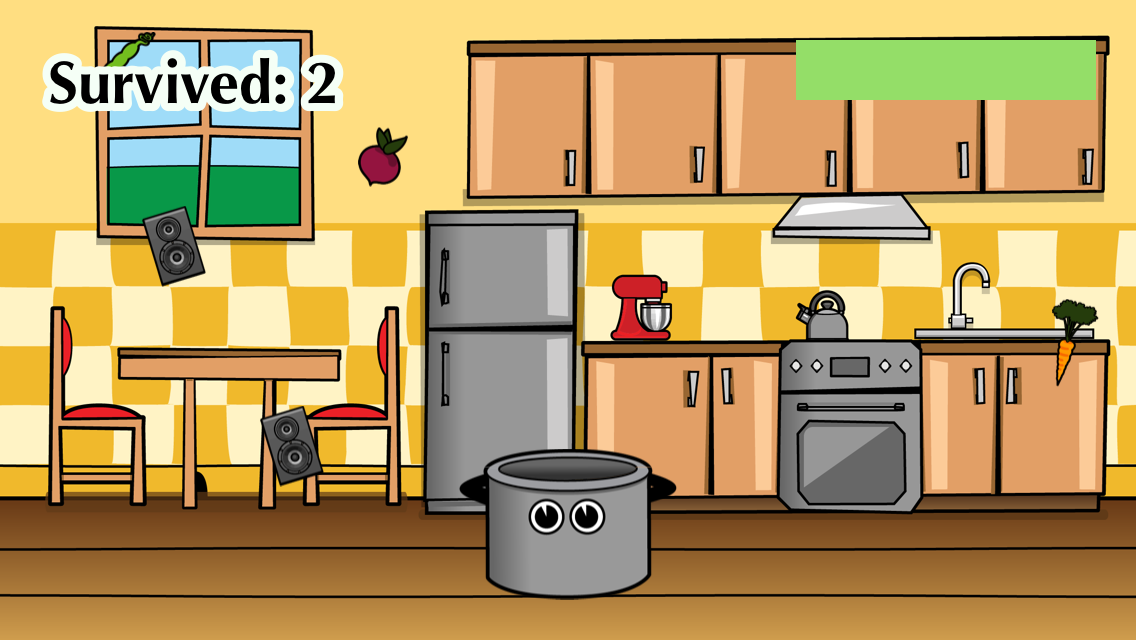
\includegraphics[width=0.5\linewidth]{images/Chapter7/endless_game_with_ui.png}
    \caption{The endless game mode features a survival time label and a health
    bar}
\end{figure}

You should see the health bar grow and shrink according to the game mode
rules that we implemented; finally all the parts have come together.

Currently the automatic transition from the main scene back to the start scene,
as soon as the game ends, is a little unexpected. It's typical for games to
present a summary after each session the player has completed. In the next section we'll add a game over
popup to our game.

\section{Adding a Game Over Popup}
Whenever a session ends, either because of a game over situation or because the
time has run out, we want to present a popup that shows the results of this
session. The popup should also provide easy ways to play the same game mode
again and to switch back to the start scene.

By the end of this section we will have built a popup that looks like this:
\begin{figure}[H]
    \centering
    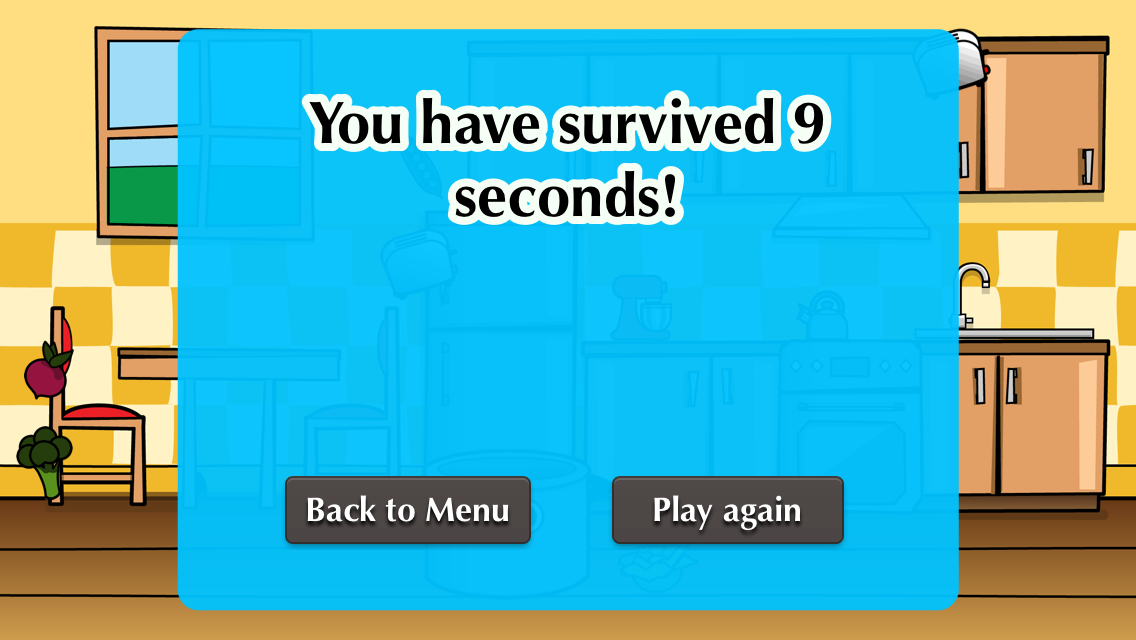
\includegraphics[width=0.5\linewidth]{images/Chapter7/game_over_popup.png}
    \caption{A popup at the end of each playing session summarizes the player's
    results}\label{fig: gameover_popup}
\end{figure}

We will get started by creating this new UI element in \SB{}, then we will work
on integrating it in code.

\subsection{Setting up the Popup in \SB{}}
We'll start by creating a new \ccbfile{} for our popup.
\begin{leftbar}
Create a new \ccbfile{} in \SB{}. Select \textit{Layer} as the type.
\textbf{Choose the size to be \textit{(400, 300)}} and name the file
\filemention{GameOverPopup}.
\end{leftbar}
We will center the popup when we present it. Centering is a lot easier when the
anchor point of the popup is at (0.5, 0.5).
\begin{leftbar}
Select the root node of \filemention{GameOverPopup} and change the
\textit{Anchor point} to (0.5, 0.5).
\end{leftbar} 
Next, we'll add the background for the popup. As you might have seen in figure
\ref{fig: gameover_popup} our popup has rounded corners. The easiest way to
accomplish rounded corners in \cocos{} is using a stretchable image.\index{Nodes!CCSprite9Slice}
 The specific type of image we want to use is called a \textit{9 slice} image. 9
 slices images are divided into stretchable and non-stretchable parts. Using 9 slices images we can
use small images and scale them to arbitrary dimensions without distorting the
non-scalable parts of the image.

Here's an illustration of how a 9 slice image works:
\begin{figure}[H]
    \centering
    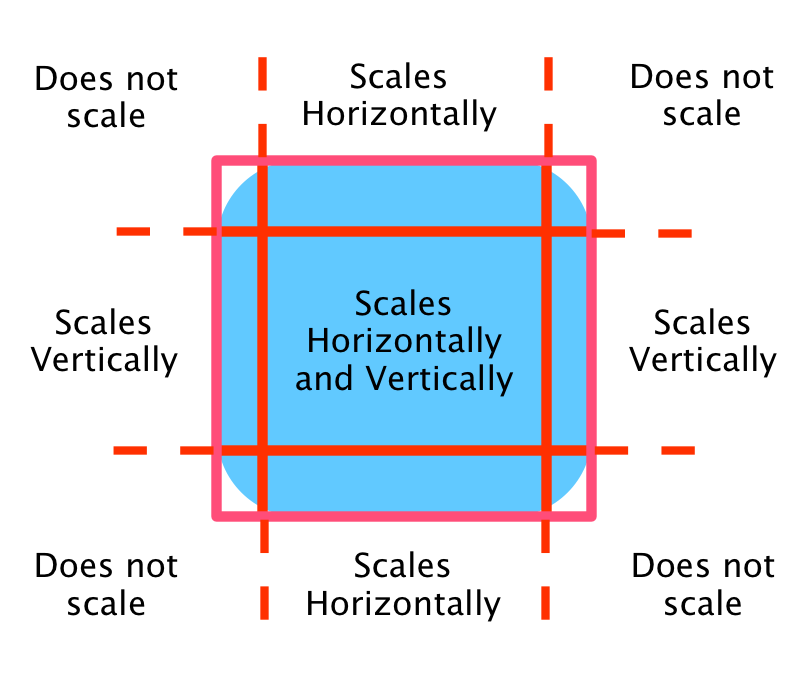
\includegraphics[width=0.5\linewidth]{images/Chapter7/9_slice.png}
    \caption{A 9 slice image is divided into stretchable and non-stretchable
    regions}
\end{figure}

In the example above we have a blue image with rounded corner. If we want to
scale that image, it's important that the corners don't get scaled, otherwise
they would be distorted. \SB{} allows us to define the scalable area of 9 slice
images, that way we can choose a scalable area that is appropriate for each
asset. The assets you have downloaded include an image with rounded corners.
We'll use that for the background of our popup.

\begin{leftbar}
Drag a \textit{Sprite 9 Slice} from the node library and add it to the root node
of \filemention{GameOverPopup.ccb}.

Set up the sprite 9 slice as following:
\begin{enumerate}
  \item Set the \textit{Position type} to \textit{percent of parent
  container} for \textit{x} and \textit{y} position
  \item Set the \textit{Position} to \textit{(50, 50)}
  \item Set the \textit{Content size type} to \textit{percent of parent
  container} for
  \textit{width} and \textit{height}
  \item Set the \textit{Width} to \textit{(100\%, 100\%)} 
  \item Set the \textit{Anchor point} to \textit{(0.5, 0.5)}
  \item Set the \textit{Sprite frame} to \textit{assets/popup-background.png}
  \item Set the \textit{Opacity} to \textit{0.95}
  \item Select a \textit{light blue} color
\end{enumerate}
\end{leftbar} 

At this point your stage should look like this:
\begin{figure}[H]
    \centering
    
\includegraphics[width=0.5\linewidth]{images/Chapter7/9_slice_setup.png}
\end{figure}

Note, that the asset \filemention{popup-background.png} has a white background.
That allows us to create a sprite with rounded corners of any color. You might
also have realized that the sprite 9 slice scales correctly without that we hat
to define a scalable and non-scalable region. That's because \SB{} provides
default values that work for many sprites. When you've selected a sprite 9 slice
you'll see the following entry in the \textit{Item properties} tab:
\begin{figure}[H]
    \centering
    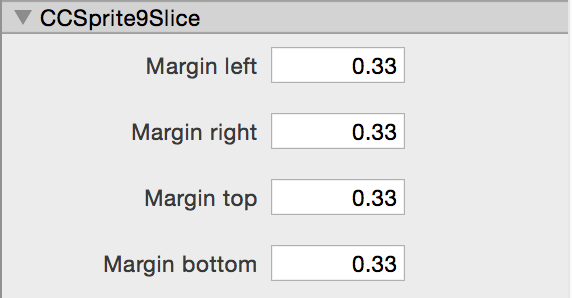
\includegraphics[width=0.5\linewidth]{images/Chapter7/9_slice_settings.png}
\end{figure}
These values are expressed in percent of the image size. This means the
non-scalable part of the image is defined as 33\% of the image size from
each edge.
These settings work well for many 9 slice image. If you ever run into problems
 with a 9 slice image (i.e. your image looks distorted), you now know where to
change these settings.

Now, we'll add the label that displays the highscore when the game is over.
We'll add this label and the two buttons as children to the sprite 9 slice
because we will be adding a little animation to the popup that will scale it up.
We want the entire popup content to scale with the sprite 9 slice.

\begin{leftbar}
Drag a \textit{Label TTF} to the stage. Drop it onto the
\textit{CCSprite9Slice} in the timeline to make the label a child of the sprite.

Set the label up as following:
\begin{enumerate}
  \item Set the \textit{Position reference corner} to \textit{Top-left}
  \item Set the \textit{X} \textit{Position type} to \textit{percentage of
  parent container}
  \item Set the \textit{Anchor Point} to \textit{(0.5, 0.5)}
  \item Set the \textit{Position} to \textit{(50, 30)}
  \item Set the label text to \textit{You have survived 10 seconds!}. This is a
  placeholder text. We'll set the actual text dynamically in code
  \item Set the \textit{Font name} to \textit{Optima-Bold}
  \item Set the \textit{Font size} to \textit{30}
  \item Set the \textit{Size type} of the \textit{Width} of the
  \textit{Dimensions} to \textit{percentage of parent container}:
  \begin{figure}[H]
    \centering
    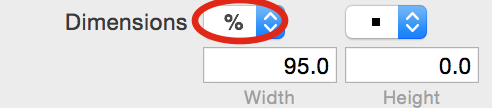
\includegraphics[width=150pt]{images/Chapter7/set_dimensions.png}
  \end{figure} 
  Labels resize dynamically based on their content, the \textit{Dimensions} size
  determines the maximum size for the label. As soon as the label reaches the
  maximum width that we define, it will start breaking into new lines
  \item Set the the Dimensions to \textit{(95, 0)}
  \item Set the horizontal alignment to \textit{Center}
  \item Set the draw color to \textit{black}
  \item Set the outline color to \textit{white}
  \item Set the outline width to \textit{4}
  \item Set up a code connection to \textit{Owner var} and name it
  \textit{gameOverPopUpHighscoreLabel}
\end{enumerate}
\end{leftbar}

By providing the \textit{owner} of the popup with access to the label we avoid
providing a custom class for the popup. Instead, whichever class displays this
popup can set itself as the owner and modify the popup appropriately. For UI
components that don't have any custom behavior I prefer this approach over
providing custom classes. Earlier we have used it as well, as we set up the
scoreboards for our different game modes.

Now we're going to create two buttons, one to play another round of the current
game mode, a second one to return to the main menu.

\begin{leftbar}
Drag a \textit{Button} to the stage. Drop it onto the
\textit{CCSprite9Slice} in the timeline to make the label a child of the sprite.

Configure the button like this:
\begin{enumerate}
  \item Set the \textit{X} \textit{Position type} to \textit{percentage of
  parent container}
  \item Set the \textit{Position} to \textit{(30, 55)}
  \item Set the \textit{Preferred size} to \textit{(120, 40)}. Buttons resize
  automatically based on their content, the preferred size determines the
  minimum size of the button
  \item Set the \textit{Title} to \textit{Back to Menu}
  \item Set the \textit{Font name} to \textit{Optima-Bold}
  \item Set up a \textit{selector} in the code connections tab. Name it
  \textit{backToMenu} and set the target to \textit{Owner}.
\end{enumerate}
\end{leftbar}

Just as we set up the \textit{code connection} of the label with the owner, we will also invoke the button callbacks on the owner
 - we want to avoid creating a custom class for this simple popup.

You can now copy this button to create the second one.
\begin{leftbar}
Copy the button that we just created. Apply the following changes:
\begin{enumerate}
  \item Change the \textit{Position reference corner} to \textit{Bottom-right}
  \item Set the \textit{Position} to \textit{(30, 55)}
  \item Change the \textit{Title} to \textit{Play again}
  \item Change the \textit{selector} in the code connections tab to
  \textit{playAgain}
\end{enumerate}
\end{leftbar}

Now the popup should look exactly as depicted in figure \ref{fig:
gameover_popup}, at the beginning of this chapter.

We're almost done with designing the popup in \SB{}. However, so far we haven't
considered how this popup is going to be presented. It would be weird if it
would suddenly appear at the end of the game, without any visual transition.
Especially iOS users are used to smooth transitions and UI elements that are
presented and dismissed with animations - our game should live up to these
standards! \SB{}'s timeline editor makes implementing this a matter of seconds.

To present the popup smoothly we will use a scale animation (very similiar to
the animation that iOS uses for its alert views). Here's what it will look like:

\begin{figure}[H]
    \centering
    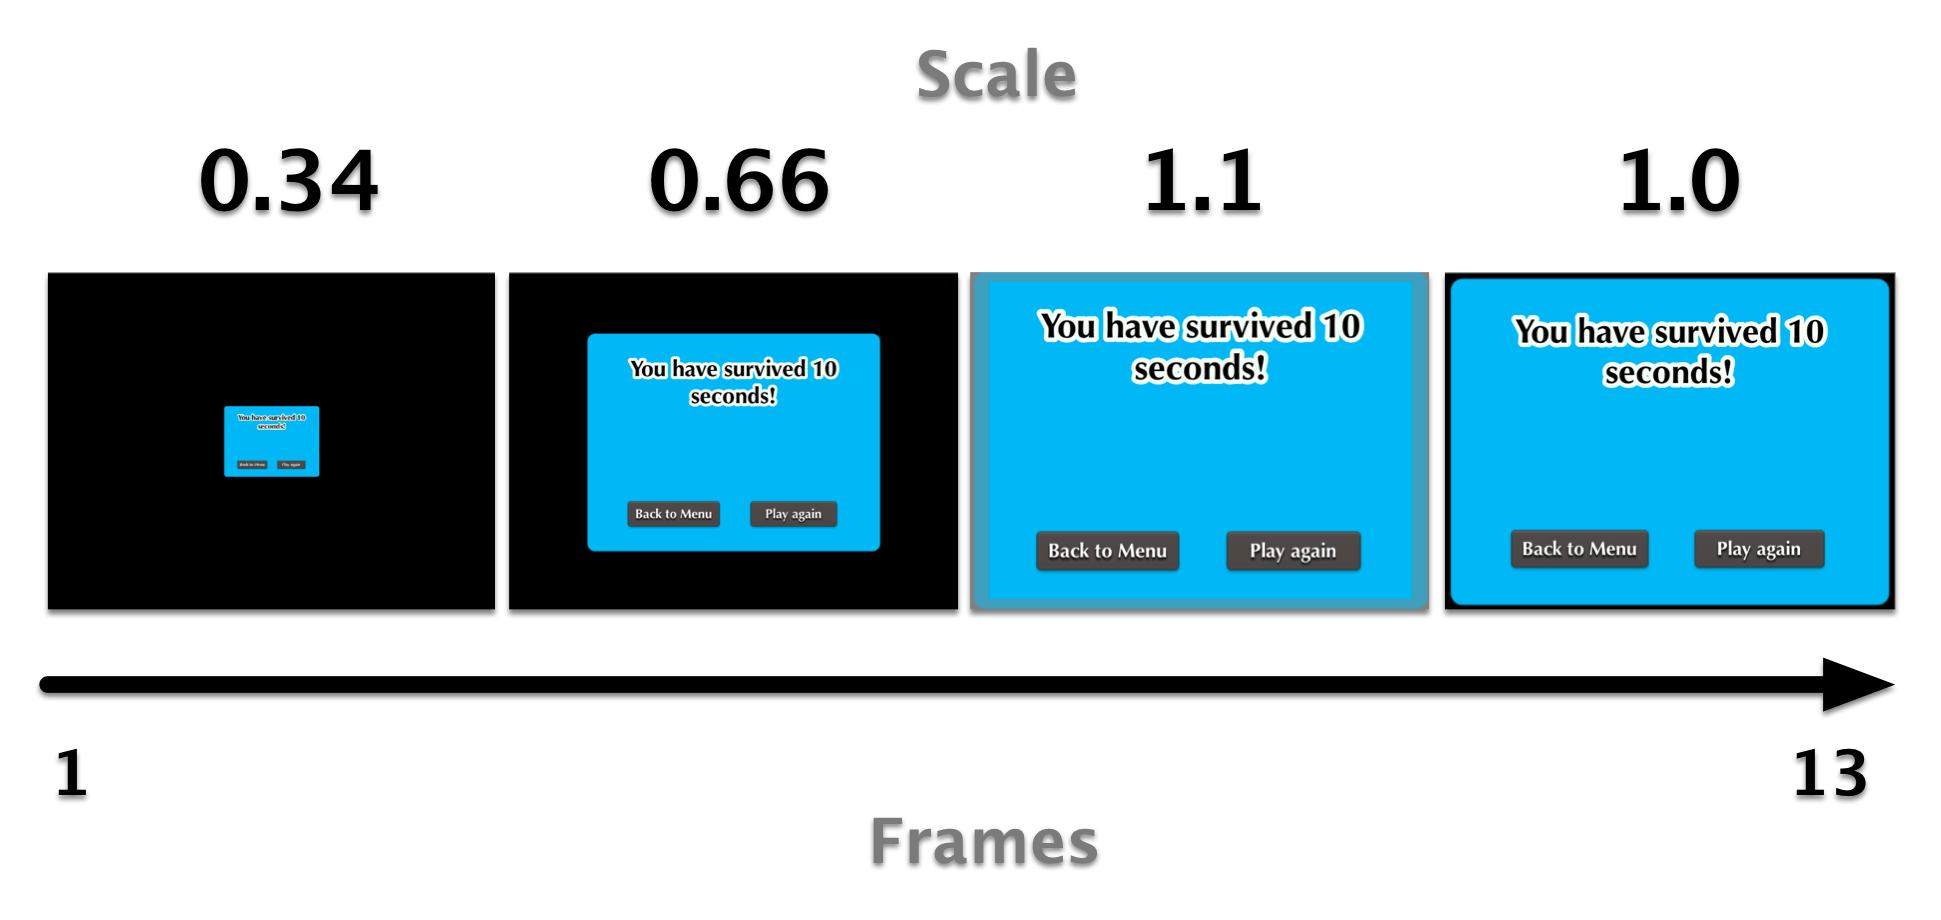
\includegraphics[width=0.75\linewidth]{images/Chapter7/popup_animation.png}
    \caption{We make the popup appear over 13 frames by animating its scale
    property}\label{fig: animate_gamover_popup}
\end{figure}

The animation will have a length of 13 frames. We will scale the popup from 0\%
to 110\% and finally to 100\% of its final size. This approach creates a nice
little bounce animation when the popup appears.

Instead of creating a new timeline we will use the \textit{Default Timeline}
that is provided by \SB{} for every \ccbfile{}. The default timeline has the
\textit{autoplay} option activated, which means that it runs as soon as the root
node of the \ccbfile{} is added to an active scene. By coincidence this is exactly
the behavior we want: as soon as the popup is added to a scene we want this
animation to play once. We can leave the \textit{autoplay} option activated and
don't need to trigger this animation in code.

Note that \SB{} does not allow us to add keyframe based animations to the root
node of \ccbfile{}, instead we will animate the \textit{CCSprite9Slice} which
has all other elements of the popup as its children.

\begin{leftbar}
Set up the animation for the popup:
\begin{enumerate}
  \item Select the \textit{CCSprite9Slice} in the timeline. Since this animation is very
short, you should use the timeline's maximum zoom level to place the keyframes
accurately. Drag the zoom lever in the top right corner all the way to the
right:
\begin{figure}[H]
    \centering
    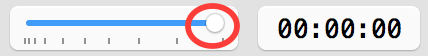
\includegraphics[width=150pt]{images/Chapter7/timeline_zoom.png}
\end{figure}

\item Now, create three keyframes for our animation. Create one at
\textit{00:00:00}, one at \textit{00:00:09} and a third one at
\textit{00:00:13}. You can create the \textit{scale} keyframes by hitting the
\textit{S} key or by using the \textit{Animation} menu.

\item Next, set the scale values by double-clicking onto each of the keyframes. As show in figure \ref{fig: animate_gamover_popup} we want the
values to be \textit{0.0}, \textit{1.0} and \textit{1.1}.
\end{enumerate}
\end{leftbar}

You can now run the animation and you should see a nice bounce effect. If you
have ever paid close attention to the animations of system elements on iOS you
will realize that something with this animation still doesn't feel exactly
right. Why?

As a default setting \SB{} uses linear interpolation between
keyframes.\index{SpriteBuilder
Timeline!Interpolation}\label{timeline_interpolation} This results in animations
that move smoothly at a constant speed. However, real life objects seldom move at a constant speed. Instead they accelerate an decelerate.
Believe it or not, the difference between a linear animation and an accelerated
one is noticeable, even if the entire animation only lasts 13 frames.

Since the developers of \cocos{} are aware of this effect, they have provided us
with a whole bunch of different interpolations. Once you have created two
keyframes and a pink bar appears between them you can select between all of
the variations by right-clicking onto the bar.

Many developers have done a good job of visualizing the different interpolation
types. Kirill Muzykov has create a nice blog post with animated diagrams of the
different interpolations that \cocos{} provides:
\url{http://kirillmuzykov.com/cocos2d-iphone-easing-examples/}.

For this animation we are going to use the \textit{Ease In} interpolation.

\begin{leftbar}
Right-click onto the segment between the \textbf{first} and the \textbf{second}
keyframe and select \textit{Ease In} as the interpolation function:
\begin{figure}[H]
    \centering
    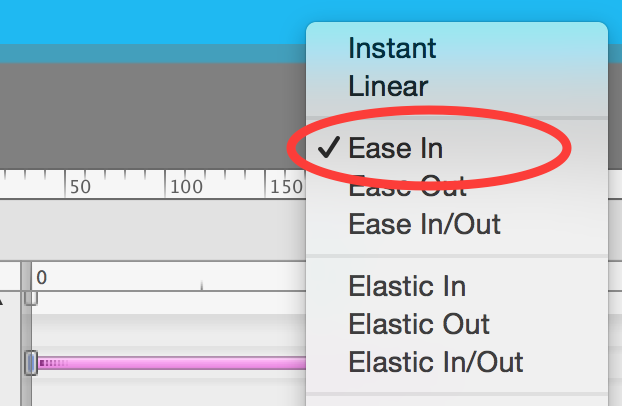
\includegraphics[width=200pt]{images/Chapter7/timeline_ease_in.png}
\end{figure}
\end{leftbar}

Now you can run the animation again. You should notice that it is looking much
better! These are the small details that catch the player's attention.

We are ready to present this popup in code!

\section{Presenting the Popup in Code}

As always, let's get started by setting up properties for the code connections
we've added in \SB{}. The code to present the popup will be part of 
\inlinecode{MainScene}. In \SB{} we've set up all code connections for the game
over popup to be connected to the \textit{Owner}. Since \inlinecode{MainScene}
will be the owner of \inlinecode{GameOverPopup} we need to add code connection
variables and callback methods there.

Let's first add the property for the label on the game over popup.
\begin{leftbar}
Add the following property to \filemention{MainScene.swift}:
\begin{lstlisting}
weak var gameOverPopUpHighscoreLabel: CCLabelTTF!
\end{lstlisting}
\end{leftbar}
This property will allow us to change the presented text on the game over popup
from within \inlinecode{MainScene}. Later we'll use it to present the final
score at the end of each game.

Our game over popup should be presented above all other content of
\inlinecode{MainScene}. We should add a new entry to the
\inlinecode{DrawingOrder} enum that places the popup at the highest z-order.

\begin{leftbar}
Extend the drawing order enum by adding a case for our new popup:
\begin{lstlisting}
enum DrawingOrder: Int {
  case GameplayElements
  case ScoreBoard
  case GameOverPopup
}
\end{lstlisting}
\end{leftbar}

Now we're set up to work on the code that adds the popup to
\inlinecode{MainScene} as soons as the game ends. We'll modify the existing
\inlinecode{gameOver} method in this step. So far \inlinecode{gameOver}
transitions back to the \inlinecode{StartScene} when the game ends. We can
remove all of that code for now.

\begin{leftbar}
Change the \inlinecode{gameOver} method, so that it no longer switches back to
the \inlinecode{StartScene}:
\begin{lstlisting}
func gameOver() {
  userInteractionEnabled = false
  isDraggingPot = false
  presentGameOverPopup()
}
\end{lstlisting}
\end{leftbar}

In the new implementation of \inlinecode{gameOver} we're disabling the user
interaction on the \inlinecode{MainScene}. This means that
\inlinecode{MainScene} will no longer receive touch events after the game ends.
Without this line it would be possible for the user to drag the pot across the screen, even though the game has ended. 
Typically you want to disable all interactions between the player and any game
elements as soon as a game ends.

In addition to disabling user interaction, we also set
\inlinecode{isDraggingPot} to \inlinecode{false}. Ongoing touch events are not
cancelled when user interaction gets disable. If a player would be
dragging the pot when the game ends, they could go one forever.
With \inlinecode{isDraggingPot} disabled, the code within
\inlinecode{touchMoved} will not be performed and the dragging is interrupted immediately.

Lastly, we're calling the \inlinecode{presentGameOverPopup} method that we
haven't implemented yet. As you'll see shortly, presenting the popup involves
quite a few lines of boilerplate code so it makes sense to bundle this
functionality into a separate method.

Let's implement \inlinecode{presentGameOverPopup} now. There aren't a lot of
new concepts involved in this method, so I'll provide the entire implementation and
will discuss the details afterwards.

\begin{leftbar}
Add the following lines to the end of the \inlinecode{MainScene} class,
directly before the closing curly braces of the class definition:
\begin{lstlisting}
func presentGameOverPopup() {
  let gameOverPopup = CCBReader.load("GameOverPopup", owner:self)
  
  // workaround because CCPositionTypeNormalized cannot be used at the moment
  // https://github.com/spritebuilder/SpriteBuilder/issues/1346
  gameOverPopup.positionType = CCPositionType(
    xUnit: .Normalized,
    yUnit: .Normalized,
    corner: .BottomLeft
  )
  
  gameOverPopup.position = ccp(0.5, 0.5)
  gameOverPopup.zOrder = DrawingOrder.GameOverPopup.rawValue
  
  gameOverPopUpHighscoreLabel.string = gameMode?.highscoreMessage()
  
  addChild(gameOverPopup)
}
\end{lstlisting}
\end{leftbar}
In the first line we are loading the \filemention{GameOverPopup.ccb} using the
\inlinecode{CCBReader}, we are setting \inlinecode{MainScene} as the owner.

Next, we're setting up the position type of the popup. We want the popup to be
presented centered on the screen. The easiest way to do that is to use the
\inlinecode{Normalized} position type (which is called \textit{Percent of
parent container} in \SB{}). We need to configure the position type in code,
because \SB{} does not support setting the position type of the root node of a
\ccbfile{}. If you select the root node of \filemention{GameOverPopup.ccb},
you'll see that the control is disabled:
\begin{figure}[H]
    \centering
    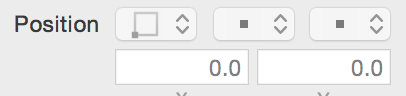
\includegraphics[width=200pt]{images/Chapter7/root_node_disabled_position_type.png}
    \caption{It isn't possible to change the position type or position of the
    root node in \SB{}}
\end{figure}
When setting the position type in code, we run into a small Swift <->
Objective-C related issue. The way that many \cocos{} constants are defined is
incompatible with Swift, these constants are not available to Swift classes.
Usually we could simply set the position type to
\inlinecode{CCPositionTypeNormalized}, but because of this issue we need to
construct the position type manually (if you are interested in the details you
can read about
the issue
here: \url{https://github.com/spritebuilder/SpriteBuilder/issues/1346}).

After we've set up the position type we center the node by setting the position
to \textit{(0.5, 0.5)} and we set the \inlinecode{zOrder} to render this popup
on top of all other game content.

Then we configure which text is displayed on the popup. We haven't implemented
this on the game mode classes yet, but we're adding a
\inlinecode{highscoreMessage} method to each game mode that will return a
suitable highscore message for the current game state. This way each game mode
can present a different message at the end of the game. This design makes it
easy to add more game modes in future. We'll discuss the
\inlinecode{highScoreMessage} method in detail as soon as we implement it.

In the next line we add the game over popup to the gameplay scene. Adding the
popup will trigger it's timeline to start playing. That will scale the popup
from 0\% to 100\% size with the animation that we have defined in \SB{}.

With this method in place we're getting close to presenting the popup! We'll
need to satisfy two more code connections: the callback methods for both
buttons on the popup.

Then we'll need to extend our game modes so that they capture a highscore that
we can display within the popup.

Let's start with the button and implement the callback for the \textit{Back to
menu} button. All this button does is bring us back to the main scene, so the
implementation is very simple.

\begin{leftbar}
Add the \inlinecode{backToMenu} method below the
\inlinecode{presentGameOverPopup} method in \filemention{MainScene.swift}:
\begin{lstlisting}
func backToMenu() {
  let startScene = CCBReader.loadAsScene("StartScene")
  let transition = CCTransition(crossFadeWithDuration: 0.7)
  CCDirector.sharedDirector().replaceScene(startScene, withTransition: transition)
}
\end{lstlisting}
\end{leftbar}
Nothing special here, this is the code that used to live in the
\inlinecode{gameOver} method - when the player hits the \textit{Back to
menu} button, we transition back to \inlinecode{StartScene}.

The \textit{Play again} button is a little bit more exciting. This is a feature
that you'll want to add to many types of games and the implementation isn't very
complicated. The easiest way to restart the game is to create a new instance of
the \inlinecode{MainScene} class and replace the currently active scene with
that new one. I've often seen beginners in game development write code to reset
different state variables in their gameplay scene, in order to start a new match
or a new round of the same game. Creating a new instance of the core gameplay
class is the simplest and most reliable way of resetting the entire state of the
game.

For this specific game there's one small gotcha that we need to avoid. The
\inlinecode{MainScene} needs to know which gameplay mode has been selected. When
a player hits the \textit{Play again} button, we want to start the \textit{same}
game mode that the player has been playing up until then. This means that as we
create a new instance of \inlinecode{MainScene}, we need to take care of
preserving the selected game mode.

With all of this in mind, let's add the \inlinecode{playAgain} method.
\begin{leftbar}
Add the \inlinecode{playAgain} method below the \inlinecode{backToMenu} method:
\begin{lstlisting}
func playAgain() {
  let mainSceneContainer = CCBReader.loadAsScene("MainScene")
  let mainScene = mainSceneContainer.children[0] as! MainScene
  mainScene.selectedGameMode = selectedGameMode
  let transition = CCTransition(crossFadeWithDuration: 0.7)
  CCDirector.sharedDirector().replaceScene(mainSceneContainer, withTransition: transition)
}
\end{lstlisting}
\end{leftbar}
Remember, when we use the \inlinecode{CCBReader.loadAsScene()} method, the
root node from the loaded \ccbfile{} is added as a child to a
\ccscene{} instance. That is why we need to access the first child of the
loaded scene to get a reference to the new \inlinecode{MainScene} instance. With that reference
at hand we set the \inlinecode{selectedGameMode} of the new \inlinecode{MainScene} to
be the same as the currently selected game mode. The rest is business as usual;
replacing the scene with an animated transition.

And that's all there is; you now know how to add a \textit{play again} feature
to your game. As you've seen it can be done with very little effort in \cocos{}!

Now we'll extend the game modes to provide individual highscore messages, so
that we have something to display on our highscore popup.

\section{Providing a Highscore for each Game Mode}
Whenever we want to extend the functionality of our game modes we should start
by adding the new features to the \inlinecode{GameMode} protocol.
\begin{leftbar}
Add the following method to the \inlinecode{GameMode} protocol:
\begin{lstlisting}
func highscoreMessage() -> String
\end{lstlisting}
\end{leftbar}
Now every game mode will be required to implement a
\inlinecode{highscoreMessage} method. Let's go ahead and add them, so we can
finally see the popup in action.

Let's start with the \inlinecode{EndlessGameMode}. When the
\inlinecode{EndlessGameMode} ends, we want to display how many seconds a player
has survived.

\begin{leftbar}
Add the following implementation of \inlinecode{highscoreMessage} to
\inlinecode{EndlessGameMode}:
\begin{lstlisting}
func highscoreMessage() -> String {
  let secondsText = Int(survivalTime) == 1 ? "second" : "seconds"
  return "You have survived \(Int(survivalTime)) \(secondsText)!"
}
\end{lstlisting}
\end{leftbar}
The most exciting part of this implementation is the ternary operator that we
use to determine whether or not we need to pluralize the term
\inlinecode{second}. 

Whenever the timed game mode ends we want to display the accomplished score. The
implementation of \inlinecode{highscoreMessage} is very similar for both game
modes.
\begin{leftbar}
Implement the \inlinecode{highscoreMessage} method in \inlinecode{TimedGameMode}
as following:
\begin{lstlisting}
func highscoreMessage() -> String {
  let pointsText = points == 1 ? "point" : "points"
  return "You have scored \(Int(points)) \(pointsText)!"
}
\end{lstlisting}
\end{leftbar}
Awesome! Now we have all the parts together to actually test our new popup. Run
the game on the simulator or on a phone, lose one of the two game modes, and see
what happens.

You should see something very similar to this:
\begin{figure}[H]
    \centering
    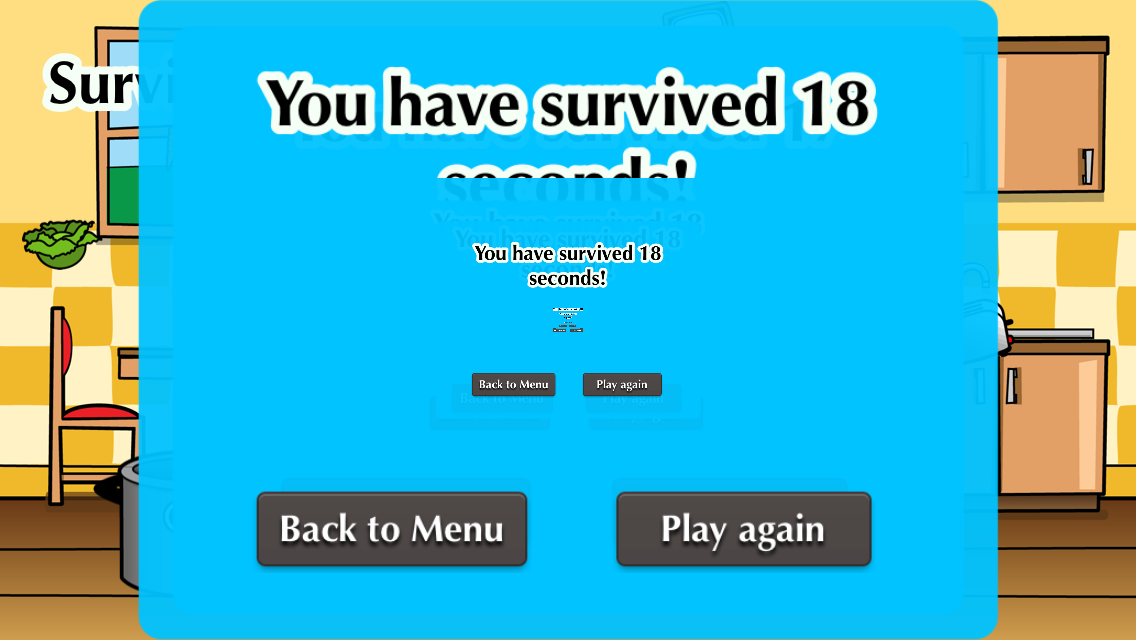
\includegraphics[width=0.75\linewidth]{images/Chapter7/endless_popups.png}
    \caption{An endless amount of popups is filling up the screen (and our
    main memory)}
\end{figure}
As soon as the game ends our popup gets presented. But not only once; new
popups are added endlessly. Why is that happening? We'll look into fixing this
in the next section.

\section{Tweaking the Game Over Popup}
The issue we are experiencing is very common among developers that are
implementing their first game over popup. What is going wrong?

We are presenting the popup from within the \inlinecode{update:} method. That
method gets called 60 times a second. We are currently not checking whether or not we've already presented the popup. 
Instead, we present a new game over popup every single frame because the game
over condition is always met. If you have the
patience to wait long enough you will experience a crash due to excessive use of
memory.

The fix for this problem is pretty straightforward. We'll add a boolean flag to
\inlinecode{MainScene} that will indicate whether we are in \textit{game over}
state or not. If we are in game over state, we will skip the entire
\inlinecode{update:} method. That way we will no longer check if the game over
condition is met which means we'll no longer present an endless amount of
popups. This approach has another advantage: since we've implemented all object
movement inside of the \inlinecode{update:} method, all objects will freeze as
soon as the game ends. That's the behavior that most players expect. 

Let's add a new property to reflect the state of the game.

\begin{leftbar}
Add the following property to \inlinecode{MainScene}:
\begin{lstlisting}
private var gameEnded = false
\end{lstlisting}
\end{leftbar}

By default, \inlinecode{gameEnded} is \inlinecode{false}, as soon as the game
ends we'll set it to \inlinecode{true}. The most convenient place to set the
flag is inside of the \inlinecode{gameOver} method, since this method is called
as soon as the game ends.

\begin{leftbar}
Modify the \inlinecode{gameOver} method of \inlinecode{MainScene} to look as
following:
\begin{lstlisting}
func gameOver() {
  (*@\colorbox{light-gray}{gameEnded = true}@*)
  userInteractionEnabled = false
  isDraggingPot = false
  presentGameOverPopup()
}
\end{lstlisting}
\end{leftbar}

Now, we'll also need to modify the \inlinecode{update:} method to check for this
flag.
\begin{leftbar}
Add the following statements to the beginning of the \inlinecode{update:}
method:
\begin{lstlisting}
override func update(delta: CCTime) {
  if (gameEnded) {
    return
  }
...
}
\end{lstlisting}
\end{leftbar}
If the \inlinecode{isGameOver} flag is set we immediately return from the
\inlinecode{update:} method, without performing any game logic.

Now you can run the game again, and you should notice that our issue is fixed.

However, there's another small problem we should work on. When the game ends and
the popup appears, we have multiple score displays on screen. The popup informs
us about the final score, and in the background, behind the popup, we can see
the scoreboard that is displayed while the game is running.

\begin{figure}[H]
    \centering
    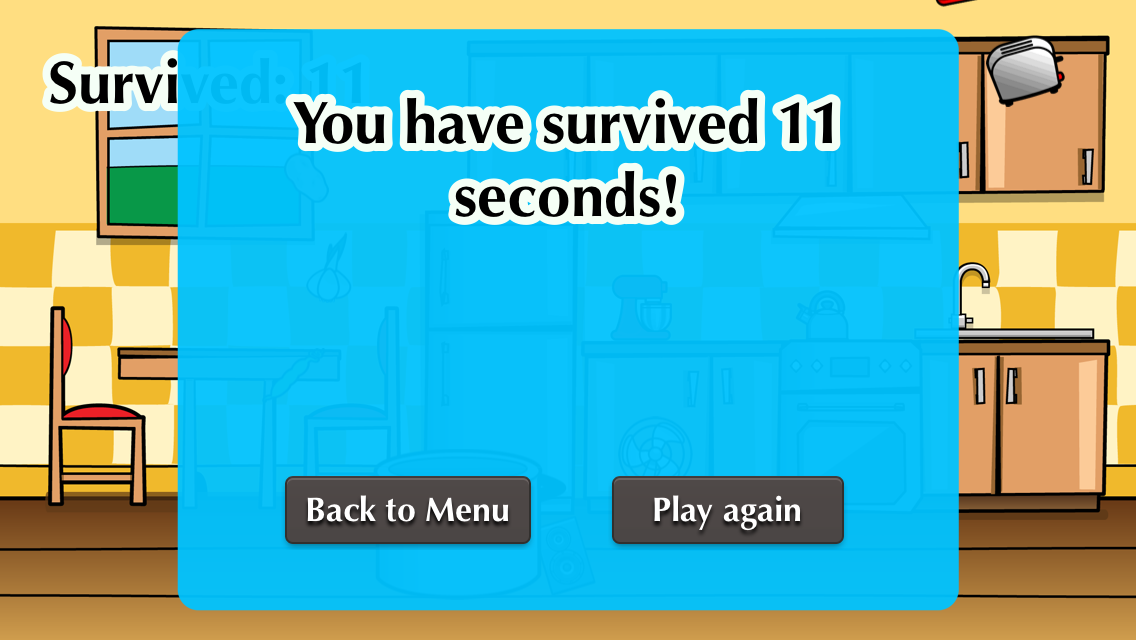
\includegraphics[width=0.75\linewidth]{images/Chapter7/no_ui_fadeout_popup.png}
    \caption{The player is confronted with score information in two places. The
    popup and the scoreboard contain the same information.}
\end{figure}

To fix this, we'll hide the scoreboard UI as soon as the game over popup is
presented. We'll extend the \inlinecode{presentGameOverPopup} method to
implement this.

\begin{leftbar}
Add the following three lines to the end of \inlinecode{presentGameOverPopup}:
\begin{lstlisting}
func presentGameOverPopup() {
  ...  
  let fadeOutAction = CCActionFadeOut.actionWithDuration(0.3) as CCAction
  gameMode?.userInterface.cascadeOpacityEnabled = true
  gameMode?.userInterface.runAction(fadeOutAction)
}
\end{lstlisting}
\end{leftbar}

Animated appearances and disappearances always look a lot better than unanimated
ones. With \cocos{} we can accomplish visual effects with only a few lines of
code, so we fade out the scoreboard UI instead of simply making it invisible.

With this code in place you can test the game once again. Now you should see a
nicely presented popup with no duplicate information displayed behind it:

\begin{figure}[H]
    \centering
    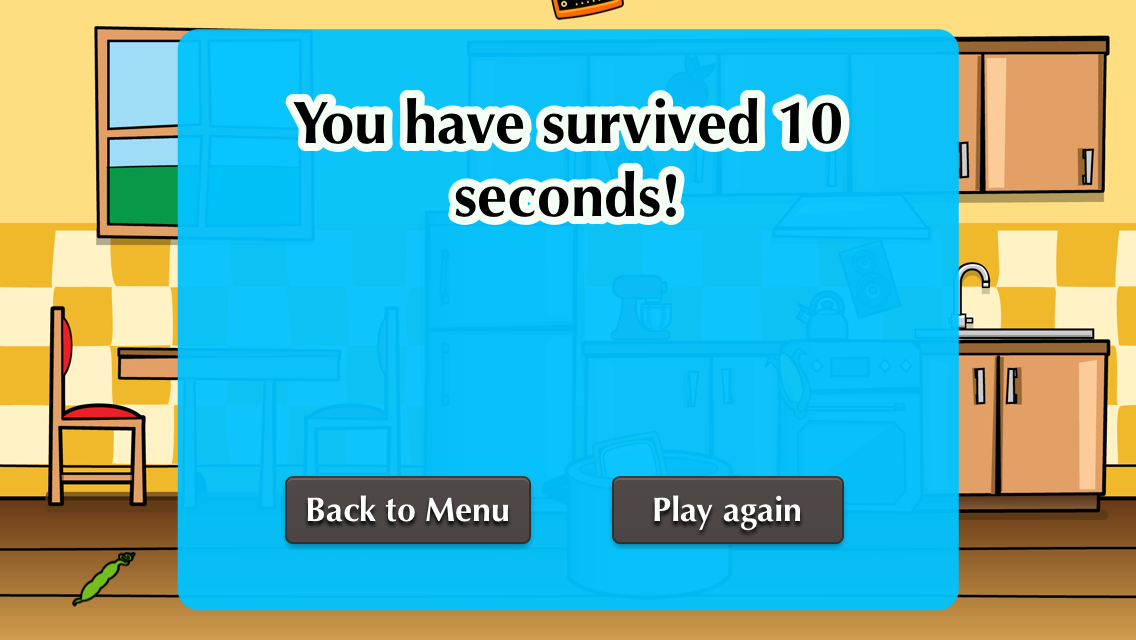
\includegraphics[width=0.75\linewidth]{images/Chapter7/ui_fadeout_popup.png}
    \caption{Without the score information in \inlinecode{MainScene} this popup
    looks more polished}
\end{figure}

\section{Summary} 

Well done! In this chapter you have learned a lot about user interfaces in \SB{}
and \cocos{}. You know how to use scroll views, how to present popups and
connect them to code efficiently and you've also learned how to implement a
restart mechanism. Additionally we've spoken a lot about code design in this
chapter. We have focused on creating this game in a way that decouples game
modes from the actual gameplay. With this design it is very easy to add more
game modes in future, and the lessons learned from this approach should apply to
many of your original games as well.

In the next chapter we will look at how we can store highscores for this game.
It is crucial to make your games competitive and to implement ways for players
to track their progress as they play your game over longer periods of time. It's
one of the best ways of keeping players engaged with your products.

\subsection{Grab the Source Code}
You can find the Source Code for this chapter on GitHub:
\url{https://github.com/SpriteBuilder-Book/Code/tree/master/Chapter6/}.